\documentclass[a4paper,12pt,table]{article}

\usepackage[left=3cm,top=2cm,right=3cm,bottom=2cm,nohead]{geometry} 


\usepackage[utf8]{inputenc}
\usepackage{polski}
\usepackage{pbox}
\usepackage[table,xcdraw]{xcolor}
\usepackage[inline]{enumitem}   
\usepackage{multirow}
\usepackage[export]{adjustbox}
\usepackage{tabularx}
\usepackage{enumitem}
\usepackage{amsmath}
\usepackage{pdfpages}
\usepackage{hyperref}
\usepackage[belowskip=-15pt,aboveskip=0pt]{caption}
\usepackage{pgfplots}

\usepackage{placeins}
\usepackage{datetime}
\usepackage{pgf}

\usepackage{tikz}

\usepackage{subfigure}
\usepackage{multicol}
\usepackage{color} %red, green, blue, yellow, cyan, magenta, black, white
\definecolor{mygreen}{RGB}{28,172,0} % color values Red, Green, Blue
\definecolor{mylilas}{RGB}{170,55,241}
\usepackage{listings}
\usepackage{amssymb}
\usepackage[T1]{fontenc}
\usepackage{libertine}



\newtheorem{twr}{Twierdzenie}
\makeatletter
% This command ignores the optional argument for itemize and enumerate lists
\newcommand{\inlineitem}[1][]{%
\ifnum\enit@type=\tw@
    {\descriptionlabel{#1}}
  \hspace{\labelsep}%
\else
  \ifnum\enit@type=\z@
       \refstepcounter{\@listctr}\fi
    \quad\@itemlabel\hspace{\labelsep}%
\fi}
\makeatother
\parindent=0pt
\lstdefinestyle{BashInputStyle}{
  language=bash,
  basicstyle=\small\sffamily,
  numbers=left,
  numberstyle=\tiny,
  numbersep=3pt,
  frame=tb,
  columns=fullflexible,
  backgroundcolor=\color{gray!20},
  linewidth=0.9\linewidth,
  xleftmargin=0.1\linewidth
}
\colorlet{punct}{red!60!black}
\definecolor{background}{HTML}{EEEEEE}
\definecolor{delim}{RGB}{20,105,176}
\colorlet{numb}{magenta!60!black}
\makeatletter
\newcommand{\lstuppercase}{\uppercase\expandafter{\expandafter\lst@token
                           \expandafter{\the\lst@token}}}
\newcommand{\lstlowercase}{\lowercase\expandafter{\expandafter\lst@token
                           \expandafter{\the\lst@token}}}
\makeatother

\lstdefinestyle{Oracle}{basicstyle=\ttfamily,
                        keywordstyle=\lstuppercase,
                        emphstyle=\itshape,
                        showstringspaces=false,
                        }
\lstdefinelanguage[Oracle]{SQL}[]{SQL}{
  morekeywords={ACCESS, MOD, NLS_DATE_FORMAT, NVL, REPLACE, SYSDATE,
                TO_CHAR, TO_NUMBER, TRUNC},
}
\definecolor{light-gray}{gray}{0.95}

\lstset{
  breaklines=true,                                     % line wrapping on
  language=SQL,
  frame=ltrb,
  framesep=5pt,
  basicstyle=\normalsize,
  keywordstyle=\ttfamily\color{green},
  identifierstyle=\ttfamily\color{blue}\bfseries,
  commentstyle=\color{Brown},
  stringstyle=\ttfamily,
  showstringspaces=ture,
  backgroundcolor=\color{light-gray},
  numbers=left
  }
  
  \lstset{language=Matlab,%
    %basicstyle=\color{red},
    breaklines=true,%
    morekeywords={matlab2tikz},
    keywordstyle=\color{blue},%
    morekeywords=[2]{1}, keywordstyle=[2]{\color{black}},
    identifierstyle=\color{black},%
    stringstyle=\color{mylilas},
    commentstyle=\color{mygreen},%
    showstringspaces=false,%without this there will be a symbol in the places where there is a space
    numbers=left,%
    numberstyle={\tiny \color{black}},% size of the numbers
    numbersep=9pt, % this defines how far the numbers are from the text
    emph=[1]{for,end,break},emphstyle=[1]\color{red}, %some words to emphasise
    %emph=[2]{word1,word2}, emphstyle=[2]{style},    
}


\lstdefinelanguage{json}{
    basicstyle=\normalfont\ttfamily,
    numbers=left,
    numberstyle=\scriptsize,
    stepnumber=1,
    numbersep=8pt,
    showstringspaces=false,
    breaklines=true,
    frame=lines,
    backgroundcolor=\color{background},
    literate=
     *{0}{{{\color{numb}0}}}{1}
      {1}{{{\color{numb}1}}}{1}
      {2}{{{\color{numb}2}}}{1}
      {3}{{{\color{numb}3}}}{1}
      {4}{{{\color{numb}4}}}{1}
      {5}{{{\color{numb}5}}}{1}
      {6}{{{\color{numb}6}}}{1}
      {7}{{{\color{numb}7}}}{1}
      {8}{{{\color{numb}8}}}{1}
      {9}{{{\color{numb}9}}}{1}
      {:}{{{\color{punct}{:}}}}{1}
      {,}{{{\color{punct}{,}}}}{1}
      {\{}{{{\color{delim}{\{}}}}{1}
      {\}}{{{\color{delim}{\}}}}}{1}
      {[}{{{\color{delim}{[}}}}{1}
      {]}{{{\color{delim}{]}}}}{1},
}
\definecolor{gray}{rgb}{0.4,0.4,0.4}
\definecolor{darkblue}{rgb}{0.0,0.0,0.6}
\definecolor{cyan}{rgb}{0.0,0.6,0.6}
\lstdefinelanguage{XML}
{
tabsize=3,
  morestring=[b]",
  morestring=[s]{>}{<},
  morecomment=[s]{<?}{?>},
  stringstyle=\color{black},
  identifierstyle=\color{darkblue},
  keywordstyle=\color{cyan},
   backgroundcolor=\color{background},
  morekeywords={xmlns,version,type}% list your attributes here
}



\newdateformat{monthyeardate}{%
  \monthname[\THEMONTH] \THEYEAR}


\begin{document}
% \renewcommand{\arraystretch}{1.8}
% \renewcommand{\arraystretch}{1.8}

\begin{titlepage}

\newcommand{\HRule}{\rule{\linewidth}{0.5mm}} % Defines a new command for the horizontal lines, change thickness here

\center % Center everything on the page
 
%----------------------------------------------------------------------------------------
%	HEADING SECTIONS
%----------------------------------------------------------------------------------------
\begin{minipage}{0.17\textwidth}
\bigskip

\includegraphics[scale=0.4]{agh}\newline
\bigskip
\end{minipage}\hfill
\begin{minipage}{0.83\textwidth}
\bigskip
\bigskip
\bigskip
\bigskip
\bigskip
\bigskip
\bigskip
\bigskip
\bigskip
\bigskip
\bigskip
\textsc{\small Akademia Górniczo-Hutnicza im. Stanisława Staszica w Krakowie}\\[0.2 cm] % Name of your university/college
{\Large Wydział Fizyki i Informatyki Stosowanej}\\
\end{minipage}
\vspace*{0mm}

\hrule width \hsize height 2pt \kern 1mm \hrule width \hsize  

 % Major heading such as course name
\vspace*{2.5 cm}
\begin{center}
{\Huge \textbf{Praca inżynierska}}
\end{center}
%----------------------------------------------------------------------------------------
%	AUTHOR SECTION
%----------------------------------------------------------------------------------------

\vspace*{1 cm}
\begin{center}
{\Large \textbf{Maciej Kubicki}}
\end{center}
\renewcommand{\sfdefault}{phv}
\begin{center}
{kierunek studiów: \textbf{informatyka stosowana}}
\end{center}

%----------------------------------------------------------------------------------------
%	TITLE SECTION
%----------------------------------------------------------------------------------------

\vspace*{2 cm}
\begin{center}
{\huge \textbf{JSON w bazie danych PostgreSQL}}
\end{center}

\begin{center}
{\large \textit{JSON in PostgreSQL database}}
\end{center}

\vspace*{1.5 cm}
{\large Opiekun: \textbf{dr inż. Grażyna Krupińska}}

% If you don't want a supervisor, uncomment the two lines below and remove the section above
%\Large \emph{Author:}\\
%John \textsc{Smith}\\[3cm] % Your name

%----------------------------------------------------------------------------------------
%	DATE SECTION
%----------------------------------------------------------------------------------------
\vspace*{6.0 cm}
{\textbf{Kraków, Styczeń 2017}}\\[3cm] % Date, change the \today to a set date if you want to be precise

%----------------------------------------------------------------------------------------
%	LOGO SECTION
%----------------------------------------------------------------------------------------

%\includegraphics{Logo}\\[1cm] % Include a department/university logo - this will require the graphicx package
 
%----------------------------------------------------------------------------------------

\vfill % Fill the rest of the page with whitespace
\newpage
\thispagestyle{empty}
\vspace*{2cm}
\vfill


\end{titlepage}



{\large Oświadczam, świadomy odpowiedzialności karnej za poświadczenie nieprawdy, że
niniejszą pracę dyplomową wykonałem osobiście i samodzielnie i nie korzystałem ze źródeł
innych niż wymienione w pracy.}\newline
\begin{minipage}{0.6\textwidth}
\qquad
\bigskip
\bigskip
\bigskip
\bigskip
\bigskip
\bigskip
\bigskip
\bigskip
\bigskip

\end{minipage}
\begin{minipage}{0.4\textwidth}
\begin{flushright}
{\large ................................................................\newline
(czytelny podpis)}
\end{flushright}

\end{minipage}

\newpage
dr inż. Grażyna Krupińska\newline
Wydział Fizyki i Informatyki Stosowanej AGH\newline
Katedra Informatyki Stosowanej i Fizyki Komputerowej

\vspace{1cm}

\textbf{Merytoryczna ocena pracy przez opiekuna:}
\parindent=10pt
\vspace*{0.5cm}\newline
\indent Celem pracy inżynierskiej Pana Macieja Kubickiego było po pierwsze przetestowanie mechanizmów
związanych z przechowywaniem dokumentów w formacie JSON w relacyjnej bazie
danych PostgreSQL. Drugim celem było porównanie wydajności mechanizmów obsługi formatu
JSON w bazie PostgreSQL z mechanizmami dostępnymi w przykładowych nierelacyjnych bazach
danych (Couchbase , MongoDB).

Po zaprezentowaniu w rozdziale pierwszym celów pracy, kolejny rozdział opisuje składnię
formatów zapisu dokumentów JSON oraz XML . Dalej znajdujemy prezentację idei relacyjnych
baz danych na przykładzie bazy PostgreSQL, oraz nierelacyjnych baz danych (baza typu kluczwartość,
bazy grafowe, bazy dokumentowe, bazy kolumnowe). Rozdział piąty poświęcony został
operatorom, indeksom, funkcjom przetwarzającym oraz funkcjom konwertującym działającym
na danych typu JSON w bazie danych PostgreSQL. Rozdział szósty przedstawia mechanizmy
przetwarzania danych typu JSON w bazach dokumentowych. Ostatni rozdział to opis oraz
podsumowanie przeprowadzonych na prezentowych bazach testów wydajnościowych.

W trakcie pracy autor wykazał się dużą samodzielnością oraz umiejętnością wykorzystania
różnych narzędzi bazodanowych. Drobne błędy w cytowaniach, oraz dosyć pobieżna analiza
wyników przeprowadzonych testów nie zmieniają pozytywnej oceny pracy.

\noindent{Końcowa ocena pracy przez recenzenta: 4.0}


\vspace*{0.15cm}
\begin{minipage}{0.5\textwidth}
\begin{center}
Data: 18.01.2017
\end{center}

\end{minipage}
\begin{minipage}{0.5\textwidth}
\begin{center}
Podpis:{\large ..........................}
\end{center}

\end{minipage}\newline

\vspace*{0.35cm}
 
 
{\scriptsize Skala ocen: 5.0 – bardzo dobra, 4.5 – plus dobra, 4.0 – dobra, 3.5 – plus dostateczna, 3.0 – dostateczna, 2.0 – niedostateczna}

\newpage
\noindent{dr inż. Mirosław Zimnoch}\newline
Wydział Fizyki i Informatyki Stosowanej AGH\newline
Katedra Zastosowań Fizyki Jądrowej
\vspace{1cm}
\newline
\textbf{Merytoryczna ocena pracy przez recenzenta:}
\vspace*{0.5cm}\newline
\indent Przedstawiona do recenzji praca inżynierska dotyczy możliwości składowania danych w formacie
JSON w relacyjnej bazie danych PostgreSQL. Autor opisał w pracy format JSON porównując
go z XML-em oraz wskazaną w tytule funkcjonalność, która została zaimplementowana
od wersji 9.2 na tle innych baz relacyjnych oraz współcześnie bardzo dynamicznie rozwijają-
cych się baz nierelacyjnych. Na uwagę zasługuje próba porównania wydajności przetwarzania
danych JSON w bazie PostgreSQL oraz dwóch systemach baz NoSQL (Couchbase i MongoDB).
Autor na wstępie przygotował odpowiednio duże zbiory danych, a następnie przeprowadził na
nich serię testów odpowiadających typowym sposobom ich przetwarzania (wyszukiwanie, grupowanie,
aktualizacja i usuwanie danych). Testy prowadzone były w seriach po 10 prób, tak
aby uzyskane wyniki były bardziej reprezentatywne, jednak autor nie pomyślał, aby porównując
uzyskane wartości średnie, przypisać im niepewności wynikające ze statystycznego rozrzutu
uzyskanych wyników. Stąd przy niewielkich różnicach czasów dla wybranych testów trudno
ocenić, czy rzeczywiście są one statystycznie istotne. Ponadto cytując literaturę autor pominął
w tekście odwołania do pozycji 4, 6 i 7. Nieprawidłowa jest też kolejność cytowania, a praca zawiera
szereg drobnych błędów. Mimo tych uchybień uważam pracę za wartościową, a uzyskane
wyniki za ciekawe.

\noindent{Końcowa ocena pracy przez recenzenta: 4.0}


\vspace*{0.15cm}
\begin{minipage}{0.5\textwidth}
\begin{center}
Data: 18.01.2017
\end{center}

\end{minipage}
\begin{minipage}{0.5\textwidth}
\begin{center}
Podpis:{\large ..........................}
\end{center}

\end{minipage}\newline

\vspace*{0.35cm}
 
 
{\scriptsize Skala ocen: 5.0 – bardzo dobra, 4.5 – plus dobra, 4.0 – dobra, 3.5 – plus dostateczna, 3.0 – dostateczna, 2.0 – niedostateczna}
\parindent=0pt
\newgeometry{
 a4paper,
 total={170mm,257mm},
 left=30mm,
 top=20mm,
 right=25mm,
 bottom=2cm,
 nohead
 }
\newpage
\tableofcontents
\newpage
%------------------------------1-------------------------------
\section{Wstęp}
\setlength{\parskip}{2\bigskipamount plus \smallskipamount minus \smallskipamount}


\indent Od początku istnienia baz danych to zapotrzebowanie rynku, czy to naukowego, czy też komercyjnego oraz postęp technologi informatycznych kształtowały ich rozwój. Pojęcie bazy danych stało się popularne we wczesnych latach sześćdziesiątych, kiedy to poszukiwano wydajnych metod dostępu do składowanych informacji. Kolejne lata to zaprezentowanie i stopniowy rozwój relacyjnego modelu, który jest stosowany do dziś. Jeszcze w końcowych latach wieku XX pojawiły się takie pojęcia jak rozproszone i obiektowe bazy danych. Początek XXI wieku to gigantyczny wzrost liczby przechowywanych informacji w związku z którym wystąpiła potrzeba szukania nowych modeli przechowywania danych oraz ich przetwarzania. Pojawiły się rozwiązania NoSQL-owe. Pojęcie to pochodzi od zwrotu non SQL (ang.\textit{ non relational }- nie relacyjne), jednak obecnie wiąże się je ze powiedzeniem angielskim - not only SQL (nie tylko relacyjne). Proces rozwoju baz danych nie jest ukierunkowany tylko w jednym kierunku. Współbieżnie następuje postęp w aspekcie takich pojęć jak hurtownie danych (ang.\textit{ Data Warehouse}, obecnie utożsamiane z nazwą \textit{Buisness Inteligence}), czy też Big Data.

\noindent{
Jedną podgałęzią wspomnianego wcześniej NoSQL-a jest model dokumentowy, który początkowo był oparty o dokumenty typu XML, jednak typ ten obecnie jest wypierany przez wydajniejsze oraz dużo bardziej wpisujące się w konwencje NoSQL, a mianowicie przez typ JSON. Celem pracy jest przedstawienie możliwości tego formatu zaimplementowanego w relacyjnej bazie danych jaką jest PostgreSQL oraz porównanie tychże narzędzi z innymi rozwiązaniami NoSQL-owymi. }

\noindent{Praca składa się z kilku części. W pierwszej przedstawiłem format JSON, wraz próbą porównania go z jego prekursorem w dziedzinie dokumentowych baz danych XML-em. W drugiej zestawiłem ze sobą model relacyjny oraz nierelacyjny baz danych. W trzeciej części prezentuję PostgreSQL w aspekcie możliwości wykorzystania JSON-a. W ostatniej części przedstawiam nierelacyjne bazy danych - Couchbase i MongoDB, a następnie zestawiam je z PostgreSQL w celu zbadania wydajności.}

\subsection{Wykorzystane oprogramowanie}
W pracy inżynierskiej używałem PostgreSQL 9.6.1, MongoDB 3.2.1, Couchbase Server Enterprise 4.5.1 oraz Python 2.7 wraz z odpowiednimi bibliotekami.
\newpage

\section{Format JSON}
Pełne rozwinięcie JSON to JavaScript Object Notation. Geneza tego formatu jest związana z pojawieniem się zapotrzebowania na lekki - wydajny, przyjazny dla użytkownika standard asynchronicznej wymiany danych między serwerem, a użytkownikiem z pominięciem dodatkowych rozszerzeń przeglądarki. Początkowo JSON był elementem JavaScript-u, jednak obecnie jest notacją niezależną. Format ten jest popularnie stosowany w implementacji AJAX-a (ang. \textit{asynchronous JavaScript and XML}), obecnie można spotkać określenie AJAJ (ang. \textit{asynchronous JavaScript and JSON}). Technologie te odnoszą się do dynamicznego odświeżania fragmentów aplikacji webowych, bez konieczności przeładowywania całej aplikacji. Wstępnie jako formę wymiany danych stosowana XML-a, jednak swoista natywność JSON-a dla JavaScriptu spowodowała to, że wypiera on XML w tym aspekcie. Kolejnymi zaletami nad XML-em są mniejszy rozmiar oraz brak ścisłych reguł odnoszących się do formatowania. Inną grupą technologii, dla które coraz powszechniejszy staje się JSON są web serwisy (ang.\textit{ web services}). Domyślnie dokumenty JSON-a zakodowane są przy pomocy UTF-8. Rozszerzenie plików zawierających tę notacje to ".json". Format JSON jest wspierany przez wiele języków programowania np. JAVA, Python i C\#. \cite{js}
\setlength{\parskip}{1\bigskipamount plus \smallskipamount minus \smallskipamount}
\subsection{Składnia i typy danych JSON-a}
Typy danych:\begin{itemize}
\item typ string - sekwencja znaków rozpoczęta i zakończona ". Pusty string jest poprawy,
\item typ numeryczny,
\item typ logiczny,
\item null,
\item tablica - może zawierać dane różnych typów, a także być pusta,
\item obiekt - rozpoczyna się od \{ i kończy na \}, zawiera pary klucz:wartość, gdzie klucz to string, a wartość może być każdym z typów. 
\end{itemize}
\setlength{\parskip}{2\bigskipamount plus \smallskipamount minus \smallskipamount}
\newpage
\subsection{Przykładowy JSON}
\begin{lstlisting}[language=json]
{
	"objectID": 1232214,
	"book": {
		"title": "Pan Tadeusz",
		"pages": 1200,
		"date": null,
		"publisher": "PolishPub",
		"author": {
			"firstName": "Adam",
			"lastName": "Mickiewicz"
		}
	},
	"isAvailable": true,
	"whoHadIt": [{
		"clientID": 1,
		"clientName": "John",
		"clientLastName": "Knox",
		"phoneNumber": "608123123"
	}, {
		"clientID": 12,
		"clientName": "Ann",
		"clientLastName": "Snow",
		"phoneNumber": "612123123"
	}, {
		"clientID": 1112,
		"clientName": "Gary",
		"clientLastName": "Cena",
		"phoneNumber": "512123123"
	}],
	"whoHasIt": null,
	"timeOfTakig": "2016-12-19 22:03:49",
	"timeOfReturning": "2016-12-25 12:03:49"
	"location": "PolRom3F";

}
\end{lstlisting}
\captionof{lstlisting}{Dokument JSON}\vspace{0.5cm}
Przykład używa wszystkich powyżej zaprezentowanych typów danych. Obiekt przestawia dokument, jaki mógłby być użyty w aplikacji obsługującej bibliotekę. Każdy obiekt ma swoje unikalne id, klucz book, zawiera "podklucze" opisujące dany egzemplarz. Klucz isAvailable to typ logiczny mówiący czy egzemplarz jest dostępny. Tablica whoHadIT zawiera obiekty trzech ostatnich osób, które wypożyczyły egzemplarz, w zależności od indeksów tablicy ustalamy kolejność. Klucz whoHasIt przechowuje osobę, która posiada aktualnie egzemplarz, jeśli jest null to egzemplarz jest w bibliotece. Obiekt też ma daty ostatniego wypożyczenia i oddania, a także sygnaturę, na której półce powinien znajdować się egzemplarz.\newpage
\subsection{Porównanie z XML-em}
\begin{lstlisting}[language=xml]
<?xml version="1.0" encoding="UTF-8" ?>
	<object ID="1232214" loc="PolRom3F" isAvailabe="true">
		<book pages = "1200">
			<title>Pan Tadeusz</title>
			<date />
			<publisher>PolishPub</publisher>
			<author>
				<firstName>Adam</firstName>
				<lastName>Mickiewicz</lastName>
			</author>
		</book>
		<whoHadIt queue="1">
			<clientID>1</clientID>
			<clientName>John</clientName>
			<clientLastName>Knox</clientLastName>
			<phoneNumber>608123123</phoneNumber>
		</whoHadIt>
		<whoHadIt queue="2">
			<clientID>12</clientID>
			<clientName>Ann</clientName>
			<clientLastName>Snow</clientLastName>
			<phoneNumber>612123123</phoneNumber>
		</whoHadIt>
		<whoHadIt queue="3">
			<clientID>1112</clientID>
			<clientName>Gary</clientName>
			<clientLastName>Cena</clientLastName>
			<phoneNumber>512123123</phoneNumber>
		</whoHadIt>
		<whoHasIt />
		<timeOfTakig>2016-12-19 22:03:49</timeOfTakig>
		<timeOfReturning>2016-12-25 12:03:49</timeOfReturning>	
	</object>
\end{lstlisting}
\captionof{lstlisting}{Dokument XML}\vspace{0.5cm}
Powyższy XML jest jednym z możliwych odpowiedników przykładowego JSON-a. Czytelność obydwu dokumentów jest zbliżona, jeśli dokument JSON-owy jest odpowiednio sformatowany. Warto zaznaczyć, że format zgodny ze specyfikacją jest warunkiem parsowania XML-a. Z tego wynika, że XML jest zawsze przejrzysty. Jeśli chodzi o JSON-a, to tam nie ma czegoś takiego jak sprawdzanie sposobu formatowania, jednak każda biblioteka obsługująca ten typ dokumentów posiada funkcje formatujące. Warto zauważyć, że dokument JSON ma rozmiar około $30\%$ mniejszy, niż XML. Obydwa formaty mają wsparcie wielu języków programowania, a także wielu dodatkowych narzędzi o podobnym zastosowaniu np. XML Schema i JSON Schema do walidacji struktury, XPath i JsonPath do przeszukiwania. Także wybór między tymi formatami jest trudny i nie da się jednoznacznie stwierdzić, który z nich jest lepszy. W różnych przypadkach lepiej może się sprawdzić albo jeden, albo drugi format.
\newpage
\section{Relacyjne i nierelacyjne bazy danych}
\subsection{Relacyjne bazy danych}
\noindent{Lata siedemdziesiąte XX wieku to początek rozwoju relacyjnego modelu jaki znamy dziś. Za pioniera tego podejścia w stosunku do danych jest Edgar F. Codd. Kolejną kluczową postacią w aspekcie tego rodzaju baz jest dr. Peter Chen, utożsamiany z modelem zależności encji - E-R (ang.\textit{ Enity-Relationship Model}).}

\noindent{W tym modelu relacyjnym najważniejsza jest relacja, którą można utożsamić z tabelą. 
 Relacja to zbiór dziedzin, z których każda składa się z nagłówka oraz treści. Odnosząc to stwierdzenie do pojęcia tabeli, możemy sprowadzić pojęcie relacji do zbioru nazw kolumn (nagłówków) oraz rekordów (treści). Każdy wiersz tabeli, czyli tak zwana krotka wyróżnia się od pozostałych za sprawą klucza głównego, składającego się z jednego, bądź większej ilości nagłówków. Istotną kwestią jest powiązanie między tabelami, które wynika ze wspomnianego wcześniej modeluj E-R. Oto możliwe połączenia:
 \begin{itemize}
 \item 1 do 1 - wiersz w relacji $R_1$ może posiadać tylko jeden odpowiadający mu wiersz w $R_2$ i na odwrót, na przykład mamy tabelę Użytkownicy i ZestawUstawień. Każdy użytkownik ma zdefiniowane swoje ustawienia i każde zdefiniowane ustawienia odnoszą się do jednego użytkownika,
 \item 1 do N - wiersz w relacji $R_1$ może posiadać jeden lub wiele powiązanych wierszy z relacji $R_2$, na przykład tabela Użytkownicy i Zdjęcia. Każdy użytkownik może posiadać wiele zdjęć.
 \item N do M - jeden lub wiele wierszy z relacji $R_1$ może być powiązanych z jednym lub wieloma wierszami relacji $R_2$ i na odwrót. Za przykład posłużyć mogą tabele Ludzie i Adresy.\end{itemize}  }
 
\noindent{Model relacyjny jest wsparty przez algebrę relacyjną. Bezpośrednio opartym na tejże algebrze jest język SQL, który służy do manipulacji i zarządzania danymi w relacyjnych bazach danych. Algebra relacyjna określa osiem podstawowych operatorów działających na relacjach.  W niektórych rozwiązaniach można spotkać dodatkowe operatory, które wynikają z tych podstawowych: 
\begin{itemize}
\item selekcja, %- wynikiem jej działania, są wiersze tabeli spełniające określone warunki,
\item projekcja,% - jako wynik zwracane wiersze uszczuplone o zadane kolumny,
\item iloczyn,% - wynikiem jest relacja, w której skład wchodzą kombinacje wszystkich możliwych par wierszy po jednym z $R_1$ i $R_2$
\item iloraz, %- mamy dwie relacje $R_1$, $R_2$ jedna jest binarna druga unarn
\item przecięcie,
\item złączenie,
\item suma,
\item iloraz.
\end{itemize}

\noindent{Aspektem, który implikuje to, że relacyjne bazy danych są nierozerwalnie związane z takim systemami jak banki, czy też sklepy jest transakcja, tak zwana ACID. Pojęcie to można rozumieć jako zbiór poleceń, które mają być wykonane na bazie, zwracający wyniki dla klienta. Zbiór ma być przetworzony kompletnie lub wcale. ACID oznacza cechy transakcji:
\begin{itemize}
\item atomowość (ang.\textit{ atomicity}) - to znaczy, że albo zostanie przetworzona w całości, albo w ogóle,
\item spójność (ang. \textit{consistency}) - baza danych przed i po transakcji pracuje poprawnie,
\item izolacja (ang. \textit{isolation}) - transakcje są od siebie odseparowane, ich instrukcje się nie przeplatają,
\item trwałość (ang. \textit{durability}) - zatwierdzona transakcja i wynikające z niej modyfikacje w bazie są trwałe. 
\end{itemize}}
\noindent{Oprogramowanie, które służą do zarządzania relacyjnymi bazami danych określa się jako SZRBD - system zarządzania relacyjną bazą danych (ang.\textit{ RDBMS - relational database management system}). Oto kilka takich systemów:\begin{itemize}[topsep=0pt]
\item Microsoft SQL Server,
\item IBM DB2,
\item MySQL,
\item PostgreSQL,
\item Oracle Database.

\end{itemize} }
\newpage
\subsection{Nierelacyjne bazy danych}
\noindent{Termin nierelacyjnych baz danych określa bardzo szeroki zakres rozwiązań technologicznych, z których każde odbiega od modelu relacyjnego w mniejszym lub większym stopniu. Pojęcie to stało się rozpoznawalne na początku XXI. wieku, jednak niektóre z rozwiązań opisanych tym słowem rozwijało się wcześniej. Postęp zagadnień związanych z NoSQL-em przede wszystkim wynikał z niedoskonałości modelu relacyjnego w pewnych kwestiach. Przykładem takiego aspektu jest sytuacja, gdy aplikacja ma współpracować z dynamicznie rozrastającą się bazą, której dane są nieustrukturyzowane, bądź ich forma się zmienia w czasie. Innym niezmiernie ważnym aspektem jest skalowalność horyzontalna, która w przypadku nierelacyjnego podejścia jest atutem. Sposób strukturyzacji w relacyjnych bazach danych zwykle ograniczał do skalowalności wertykalnej.}

\noindent{Patrząc trochę z innego punktu widzenia w ramach zestawienia ze sobą relacyjnego i nierelacyjnego podejścia warto przytoczyć teorie CAP, wedle, której jest niemożliwe pełne spełnienie trzech podstawowych założeń dla rozproszonego systemu bazodanowego, tzn. spójności (ang.\textit{ Consistency}), dostępności (ang.\textit{ Availability}) i tolerancji na podział (ang.\textit{ Partition tolerance}). Dla baz relacyjnych spójność jest cechą najistotniejszą, natomiast dla nierelacyjnych skalowalność, która wiąże się z partycjonowaniem. Podział w relacyjnych bazach danych jest czymś nietrywialnym na przykład w związku z istnieniem operatora złączenia.\cite{ll1}\cite{l1}   }

\noindent{Wyróżniamy kilka typów baz nierelacyjnych:
\begin{itemize}[topsep=0pt]
\item bazy klucz-wartość (ang. \textit{key-value stores}),
\item bazy grafowe (ang. \textit{graph stores}),
\item bazy dokumentowe (ang. \textit{document oriented database}),
\item bazy kolumnowe (ang. \textit{wide-column store}).
\end{itemize}}
\subsubsection{Baza klucz-wartość}
Jest to bardzo prosty rodzaj bazy, która może przechowywać jedynie klucz i odpowiadającą mu wartość, która może być listą krotek innej bazy, bądź listą obiektów lub prostą wartością. Rozwiązanie to przypomina słownik ze skryptowego języka Python. Istnieje wiele implementacji tego modelu. Niektóre wersje wprowadzają sortowanie kluczy, także widzimy różnice w przechowywaniu danych (RAM,dyski). Przykładem wykorzystanie takiego rodzaju bazy mogą być system obsługujący jakieś zdarzenia - klucz jako identyfikator zdarzenia, a wartość jako zbiór wszystkie informacje na temat zdarzenia. Przykładowe bazy klucz-wartość: Redis, BerkleyDB.
\subsubsection{Baza grafowa}
Grafy w nauce znajdują wiele zastosowań, okazały się również atrakcyjną strukturą danych. W bazach grafowych dane oraz ich powiązania są reprezentowane w postaci węzłów, krawędzi oraz własności. Węzeł, który można postrzegać jako obiekt jest powiązany z innym obiektem poprzez krawędź. Zarówno węzeł, jak i krawędź może mieć własności, czyli jakieś cechy je opisujące. Struktura grafu daje możliwość o wiele wydajniejszego wyszukiwania danych w wypadku wielokrotnego zagłębienia zapytania, niż w wypadku modelu relacyjnego. W celu wyekstrahowania zagnieżdżonych danych w wypadku relacyjnym konieczne jest użycie złączeń i kluczy obcych, natomiast w podejściu grafowym powiązane dane są połączone krawędziami z odpowiednią własnością i to wpływa na wydajność zapytań. Grafy w informatyce są dość powszechne i dzięki temu istnieje wiele algorytmów ułatwiających pracę z tym rodzajem bazy danych. Popularnym przykładem wykorzystania tych baz są sieci społecznościowe. Aplikacją działającą z tym rodzajem bazy jest Twitter. Przykładowe bazy grafowe: Neo4j, OrientDB, FlockDB.
\subsubsection{Baza dokumentowa}
Ten rodzaj baz można by uznać jako podgrupę, bądź rozwinięcie baz klucz-wartość, gdyż dane są tu przechowywane w jakimś pojemniku (np. Bucket, Collection) w formie dokumentów (wartość), z których każdy ma przypisany identyfikator (klucz). Arcyważny dla tych baz jest format przechowywania dokumentów. Istniej tu kilka możliwości w zależności od implementacji bazy: JSON, XML, BSON, YAML. Przechowywany dokument zwykle nie ma narzuconej struktury. Przede wszystkim ten rodzaj baz jest popularny w aplikacjach webowych, w szczególności korzystających z architektury RESTful. Przykładowe bazy dokumentowe: MongoDB, Couchbase, CouchDB, NosDB, DocumnetDB. 
\subsubsection{Baza kolumnowa}
Bazy kolumnowe wraz z dodawaniem kolejnych rekordów nie rozszerzają się w "dół", lecz w "szerz". Wynika to z faktu, że dane z kolumny są dodawane obok siebie. Taka implementacja pozwala na szybkie wykonywanie poleceń selekcji, agregacji, czy też filtracji. Z drugiej strony inne rodzaje poleceń mogą być wolniejsze od analogicznych w modelu relacyjnym. Ten rodzaj baz korzysta z normalnego odpowiednika SQL. Fakt szybkiego wykonywania poleceń, powoduje, że bazy kolumnowe powszechnie są wykorzystywane w analizie danych. Przykładowe bazy kolumnowe: Cassandra, HBase.
\newpage
\section{PostgreSQL}
PostgreSQL jest dynamicznie rozwijającym się systemem zarządzania relacyjną bazą danych (SZRBD), który jest darmowy. Jak sama nazwa wskazuje system jest zgodny ze standardem SQL. Postgres ma również pewne znamiona obiektowej bazy danych. Ważną cechą tego oprogramowania jest dostępność na wiele systemów operacyjnych oraz architektur. Kilkukrotnie w ciągu roku wydawane są nowe wersje rozszerzające funkcjonalność, bądź też udoskonalające już zaimplementowane rozwiązania.  
\subsection{Funkcjonalność}
Dane w Postgresie są przechowywane w zdefiniowanych przez użytkownika tabelach. SZBZ umożliwia tworzenie triggerów, widoków, indeksów, własnych typów danych, czy też własnych funkcji. Do ich tworzenia użytkownik ma w dyspozycji wiele języków programowania.
\begin{center}

  \begin{tabular}{ | c | c | }
    \hline
    \textbf{Ogranicznik} & \textbf{Wartość} \\ \hline
    Maksymalny rozmiar bazy danych & brak ograniczenia \\ \hline
    Maksymalna ilość wierszy tabeli & brak ograniczenia  \\ \hline
    Maksymalny rozmiar tabeli & $32\left[TB\right]$\\ \hline
    Maksymalny rozmiar wiersza & $1.6\left[TB\right]$\\ \hline
    Maksymalny rozmiar pola & $1\left[GB\right]$ \\
    \hline
    
  \end{tabular}
\captionof{table}{Tabela ograniczeń dla PostgreSQL \cite{p} }  
\end{center}


 Do łatwego obsługiwania serwera istnieje kilka aplikacji, między innymi: PgAdmin, psql, phpPgAdmin.
\subsection{Typy json i jsonb}
Między kilkudziesięcioma innymi typami od wersji 9.2 pojawił się typ json, a od wersji 9.4 jsonb. Obydwie struktury służą do zapisu dokumentów w formacie JSON. Podstawową różnicą miedzy nimi jest sposób przechowywania. Mianowicie pierwszy z nich jest zapisany jako dokładna kopia parametru wejściowego. Natomiast drugi z typów jest przechowywany w formie binarnej (BSON). BSON jest binarnym odpowiednikiem JSON-a, z minimalnymi rozwinięciami, na przykład BSON wspiera o kilka więcej typów danych - typ data, czy też wyrażenie regularne. Zarówno typ json i jsonb narzuca sprawdzenie zgodności danych z formatem JSON. Zmienne typowe dla JSON-a użyte w dokumencie są konwertowane do odpowiadającym im typów PostgreSQL.\cite{p}\setlength{\parskip}{1.5\bigskipamount plus \smallskipamount minus \smallskipamount}
\begin{center}

  \begin{tabular}{ | c | c | }
    \hline
    \textbf{Typ JSON} & \textbf{Typ PostgreSQL} \\ \hline
    numeryczny & numeric \\ \hline
   	string & text  \\ \hline
    logiczny & boolean\\ \hline
    null & (none)\\ 
    \hline
    \end{tabular}
\captionof{table}{Schemat konwersji typów}  
\end{center}
\setlength{\parskip}{2\bigskipamount plus \smallskipamount minus \smallskipamount}
Ze sposobu przechowywanie tych typów wynika to, że typ json jest szybszy do zapisu, niż jsonb, jednak jest wolniejszy w przetwarzaniu, gdyż jest parsowany przy każdym użyciu. Dodatkowym atutem wersji binarnej jest możliwość tworzenia indeksów na kluczach wewnątrz dokumentu. \cite{p}
\subsection{Dane testowe}
Do przedstawienia możliwości użycia formatu JSON w PostgreSQL przygotowałem dwa zestawy danych. Pierwszy zestaw został wygenerowany na podstawie AdvenutreWorks2008 z Microsoft SQL Server. Oto kod, który wygenerował zbiór 18798 dokumentów JSON. 
\begin{lstlisting}[language=Python]
from DatabasePrepartion import *
import pyodbc 
cnxn = pyodbc.connect('DRIVER={SQL Server};SERVER=localhost\SQLEXPRESS;DATABASE=AdventureWorks2008;')
cursor = cnxn.cursor()
cursor.execute("SELECT e.EmailAddress, pp.FirstName, ISNULL(pp.MiddleName,'') AS MiddleName, pp.LastName, p.BusinessEntityID,[AddressLine1],ISNULL([AddressLine2],'') AS AddressLine2,[City],[PostalCode] FROM [AdventureWorks2008].[Person].[Address] a,[AdventureWorks2008].[Person].[EmailAddress] e, [AdventureWorks2008].[Person].[BusinessEntityAddress] p, [AdventureWorks2008].[Person].[Person] pp WHERE p.AddressID = a.AddressID and pp.BusinessEntityID=p.BusinessEntityID and e.BusinessEntityID=pp.BusinessEntityID;")
rows = cursor.fetchall()

with open('person.json','w') as pl:
	for row in rows:
		if is_json(to_json(row) ):
			pl.write(to_json(row,False)+'\n')
\end{lstlisting}
\captionof{lstlisting}{Generowanie dokumentów JSON}\vspace{0.5cm}
Funkcja to\_json na podstawie wyniku wiersza generuje dokument JSON. Struktura wygenerowanych dokumentów nie jest jednakowa. Mianowicie nie każdy człowiek (odpowiadający mu dokument) posiada klucz MiddleName oraz address\_line2. Dodatkowo liczba adresów e-mail przypisanych do osoby może wynosić 0,1,2.
\newpage
Oto przykładowy dokument:
\begin{lstlisting}[language=JSON]
{
	"person": {
		"personID": 12,
		"FirstName": "Thierry",
		"MiddleName": "B",
		"LastName": "DHers"
	},
	"addres": {
		"city": "Bothell",
		"addres_line1": "1970 Napa Ct.",
		"postal_code": "98011"
	},
	"email": ["thierry0@adventure-works.com", "DHers12@mail.com"]
}
\end{lstlisting}
\captionof{lstlisting}{Wygenerowany dokument JSON}\vspace{0.5cm}
Tworzę tablice dla typu json i jsonb, a następnie wypełniam je:
\begin{lstlisting}[language=SQL]
CREATE TABLE PersonJSONB (
  "ObjectID" SERIAL   NOT NULL ,
  data JSONB NOT NULL,
PRIMARY KEY("ObjectID"));
CREATE TABLE PersonJSON(
  "ObjectID" serial NOT NULL,
  data JSON NOT NULL,
PRIMARY KEY ("ObjectID"));
\end{lstlisting}
\captionof{lstlisting}{Tworzenie tabeli w PostgreSQL z typami jsonb i json}\vspace{0.5cm}
Drugi zestaw obejmuję prostą tabelkę:
\begin{lstlisting}[language=SQL]
CREATE TYPE Gender AS ENUM('M','F');
CREATE TABLE Users (
  idUsers SERIAL   NOT NULL ,
  username VARCHAR(20)   NOT NULL ,
  password VARCHAR(255)   NOT NULL ,
  mail VARCHAR(255)   NOT NULL ,
  Name VARCHAR   NOT NULL ,
  Surname VARCHAR   NOT NULL ,
  town VARCHAR(20)   NOT NULL ,
  gender Gender   NOT NULL ,
  country VARCHAR(255) NOT NULL,
PRIMARY KEY(idUsers));
\end{lstlisting}
\captionof{lstlisting}{Tworzenie tabeli z drugim zestawem danych}\vspace{0.5cm}
\setlength{\parskip}{0.5\bigskipamount plus \smallskipamount minus \smallskipamount}
\newpage
\subsection{Operatory JSON}
PostgreSQL udostępnia kilkanaście operatorów dla typu jsonb, tylko część z nich działa na json. Pierwsza grupa operatorów działa na obu typach i ich działanie skoncentrowane jest na przeszukiwaniu dokumentu JSON. 
\begin{itemize}
\item json / jsonb \,-$>$\, 'klucz' / indeks
\item json / jsonb\, -$\gg$\, 'klucz' / indeks
\item json / jsonb\, \#$> $\,'{ścieżka}'
\item json / jsonb\, \#$\gg$\, '{ścieżka}'
\end{itemize}
Operatory z podwójnym $>$ zwracają wynik jako text, natomiast z pojedyńczym $>$ w tym typie co lewa strona operatora (jsonb/json).


\subsubsection*{Przykład 1.}
\setlength{\intextsep}{15pt plus 2pt minus 2pt}
\begin{lstlisting}[language=SQL,basicstyle=\footnotesize]
SELECT "ObjectID", data->'person'->>'LastName' AS Surname FROM personjsonb WHERE data->'person'->>'LastName' LIKE 'T%' LIMIT 5;
\end{lstlisting}
\captionof{lstlisting}{Przykład 1.}\vspace{0.5cm}
\begin{figure}[h]
\begin{center}
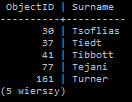
\includegraphics[scale=1.1]{sc/1}
\end{center}
\caption{Wynik zapytania z przykładu 1.}
\end{figure}

Na przykładzie widzimy użycie i operatora -$>$ i -$\gg$, w miejscu gdzie zwracamy Surname moglibyśmy użyć -$>$, jednak zwrócone nazwiska były by w cudzysłowach. Natomiast przy operatorze LIKE musimy użyć -$\gg$, by zwrócić text, ponieważ operator LIKE działa na wartości tekstowej.
\subsubsection*{Przykład 2.}
\begin{lstlisting}[language=SQL,basicstyle=\footnotesize]
SELECT max(cast(data->'person'->>'personID' AS int)) FROM personjsonb;
\end{lstlisting}
\captionof{lstlisting}{Przykład 2.}\vspace{0.5cm}
\begin{figure}[h]
\begin{center}
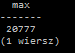
\includegraphics[scale=1.1]{sc/2}
\end{center}
\caption{Wynik zapytania z przykładu 2.}
\end{figure}%
Na przykładzie widzimy użycie i operatora -$>$ i -$\gg$, dodatkowo dodaję rzutowanie i funkcję agregującą max. Funkcjonalność typowa dla SQL współgra z typami do obsługi JSON.\newpage
\subsubsection*{Przykład 3.}
\begin{lstlisting}[language=SQL,basicstyle=\footnotesize]
SELECT data #> '{person,LastName}' AS NAME, COUNT(*) FROM public.personjsonb GROUP BY NAME;
\end{lstlisting}
\captionof{lstlisting}{Przykład 3.}\vspace{0.5cm}
\begin{figure}[h]
\begin{center}
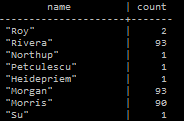
\includegraphics[scale=0.9]{sc/3}
\end{center}
\caption{Fragment wyniku zapytania z przykładu 3.}
\end{figure}%
W tym przykładzie widzimy przeszukiwanie przy pomocy \#$>$ i dodane grupowanie po nazwisku.

\subsubsection*{Przykład 4.}

\begin{lstlisting}[language=SQL,basicstyle=\footnotesize]
SELECT data->'email'->0 AS FirstEmail FROM public.personjsonb WHERE jsonb_array_length(data->'email')=1 LIMIT 3;
\end{lstlisting}
\captionof{lstlisting}{Przykład 4.}\vspace{0.5cm}
\begin{figure}[h]
\begin{center}
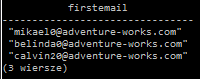
\includegraphics[scale=1]{sc/4}

\end{center}
\caption{Wynik zapytania z przykładu 4.}
\end{figure}%
Tutaj jest jeszcze przeszukiwanie dokumentu z odwołaniem się do indeksu tablicy.
\subsubsection*{Przykład 5.}
\begin{lstlisting}[language=SQL,basicstyle=\footnotesize]
SELECT DISTINCT data->'address'->'city' AS City FROM personjsonb ORDER BY City ASC;
\end{lstlisting}
\captionof{lstlisting}{Przykład 5.}\vspace{0.5cm}
\begin{figure}[h]
\begin{center}
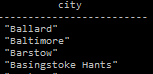
\includegraphics[scale=1]{sc/5}
\end{center}
\caption{Fragment wyniku zapytania z przykładu 5.}

\end{figure}%
Tu mamy wyszukanie unikalnych nazw miast z użyciem sortowania.\newline


\noindent{Druga grupa operatorów działa już tylko na jsonb. Ich działanie polega na sprawdzeniu zawierania się, łączeniu obiektów, a także uszczuplaniu obiektów. Wewnątrz obiektu JSON poprawnym typem jest inny obiekt JSON, a więc możliwe jest przypisanie go do klucza lub dodanie go do tablicy - zagnieżdżanie dokumentów. Na przykładzie dokumentów JSON znajdujących się w pierwszym zestawie testowym stwierdzenie zerowy poziom zagłębienia odnosi się do kluczy "person", "address", ("email"). }

\newpage
\begin{itemize}
\item jsonb \, @$>$ \,($<$@) \, jsonb - sprawdzenie czy lewy (prawy) jsonb zawiera się w prawym (lewym) w zerowym poziomie zagłębienia dokumentu,
\item jsonb\, ?\, 'klucz' - czy istnieje klucz jsonb w zerowym poziomie zagłębienia dokumentu,
\item jsonb\, ?|\,(?\&)\, 'klucze[]' - czy któryś z kluczy (wszystkie klucze) jest (są) zawarty (zawarte) w jsonb w zerowym poziomie zagłębienia dokumentu,
\item  jsonb \,-\, indeks \inlineitem jsonb \,-\, 'klucz' \inlineitem jsonb\, \#-\, '{scieżka}' - uszczuplenie obiektu o element o danym indeksie, kluczu, lub o zadanej ścieżce
\end{itemize}
\subsubsection*{Przykład 1.}
\begin{lstlisting}[language=SQL,basicstyle=\footnotesize]
SELECT count(data) FROM public.personjsonb WHERE data ? 'email';
SELECT count(data) FROM public.personjsonb WHERE data ?| array['person','address','email'];
SELECT count(data) FROM public.personjsonb WHERE data ?& array['person','address','email'];
\end{lstlisting}
\captionof{lstlisting}{Przykład 1.}\vspace{0.5cm}
Trzy zapytania pokazują przykładowe wykorzystanie operatorów zawierania. W pierwszym wypadku zliczam wszystkie dokumenty gdzie jest klucz 'email' w zerowym poziomie zagłębienia. W kolejnym zliczam te, które zawierają co najmniej jeden z kluczy z tablicy w zerowym poziomie zagłębienia, a w ostatnim te, które posiadają wszystkie klucze z tablicy na tym poziomie. Dane stworzyłem w taki sposób, że wszystkie dokumenty mają 'person' i 'address', a więc pierwsze i ostatnie zapytanie powinno dać taki sam wynik, a środkowe liczbę wszystkich dokumentów. Wyniki powyższych zapytań to: 12516, 18798, 12516.
\subsubsection*{Przykład 2.}
\begin{lstlisting}[language=SQL,basicstyle=\footnotesize]
SELECT jsonb_pretty(data #- '{"address","postal_code"}') FROM public.personjsonb WHERE "ObjectID"=1921;
\end{lstlisting}
\captionof{lstlisting}{Przykład 2.}\vspace{0.5cm}
\begin{figure}[h]
\begin{center}
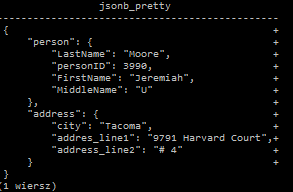
\includegraphics[scale=1]{sc/24}
\end{center}
\caption{Wynik zapytania z przykładu 2.}
\end{figure}%
Powyższy przykład pokazuje użycie operatora \#-, aby pozbyć się niechcianego pola w dokumencie.\newpage
\subsubsection*{Przykład 3.}
\begin{lstlisting}[language=SQL,basicstyle=\footnotesize]
BEGIN TRANSACTION;
SELECT jsonb_pretty(data) FROM public.personjsonb WHERE "ObjectID"=1922;
UPDATE public.personjsonb SET data = (SELECT data #- '{"email"}' || '{"email": ["newmail@hotmail.com"]}'::jsonb  FROM public.personjsonb WHERE "ObjectID"=1922) WHERE "ObjectID"=1922;
SELECT jsonb_pretty(data) FROM public.personjsonb WHERE "ObjectID"=1922;
ROLLBACK;
\end{lstlisting}
\captionof{lstlisting}{Przykład 3.}\vspace{0.65cm}
\begin{minipage}{0.5\textwidth}
\makeatletter
\def\@captype{figure}
\makeatother
\begin{center}
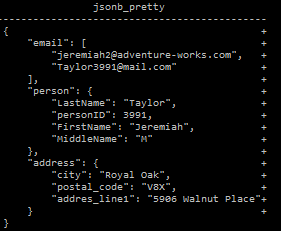
\includegraphics[scale=1]{sc/25}
\caption{Przed modyfikacją}
\end{center}

\end{minipage}
\begin{minipage}{0.5\textwidth}
\makeatletter
\def\@captype{figure}
\makeatother
\begin{center}
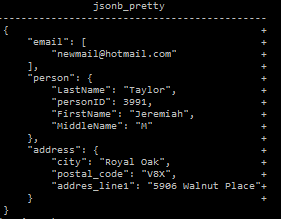
\includegraphics[scale=1]{sc/26}
\caption{Po modyfikacji}

\end{center}

\end{minipage}
\vspace{0.5cm}

Ten przykład przedstawia przeprowadzenie modyfikacji dokumentu JSON. Kasuję wszystkie adresy mailowe z wybranego dokumentu i dodaję nowy. Używam tu operatorów \#- do skasowania i || do dodania nowego adresu (w praktyce do połączenia dwóch obiektów jsonb).
\setlength{\parskip}{1\bigskipamount plus \smallskipamount minus \smallskipamount}

\newpage

\subsection{Funkcje przetwarzające dokument JSON}
%PostgreSQL wraz z udostępnianiem kolejnych wersji swojego oprogramowania rozwija dostępną funkcjonalność.
Obecnie mamy dostępne kilkadziesiąt funkcji działających na typie json i jsonb. Pierwsza grupa to tak zwane funkcje przetwarzające. Jest ich kilkanaście dla jsonb i o kilka mniej dla json. Funkcje dla typu binarnego zaczynają się od jsonb\_, a dla drugiego typu od json\_. Na przykład:
jsonb\_array\_length
i
json\_array\_length.
Wszystkie funkcje dla dokumentów przechowywanych jako json mają odpowiedniki swoich funkcji dla jsonb. Do zadań funkcji przetwarzających należy wyekstrahowanie pewnych informacji, zmiana sposobu prezentacji dokumentu, a także zmiany w strukturze tego dokumentu - dodawanie elementów, czy też zmiana aktualnych. Oto prezentacja kilku przykładów:
\setlength{\parskip}{0.5\bigskipamount plus \smallskipamount minus \smallskipamount}
\setlength{\intextsep}{15pt plus 2pt minus 2pt}
\subsubsection*{Przykład 1.}
\begin{lstlisting}[language=SQL,basicstyle=\footnotesize]
SELECT jsonb_pretty(data) FROM public.personjsonb WHERE jsonb_array_length(data->'email') = 2 LIMIT 1;
\end{lstlisting}
\captionof{lstlisting}{Przykład 1.}\vspace{0.5cm}
\begin{figure}[h]
\begin{center}
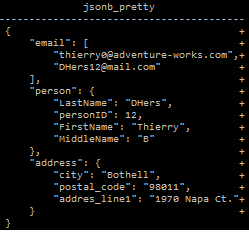
\includegraphics[scale=0.8]{sc/31}
\end{center}
\caption{Wynik zapytania z przykładu 1.}
\end{figure}%
Powyżej widzimy użycie dwóch funkcji, które już wcześniej się pojawiły - jsonb\_pretty (dostępna tylko dla jsonb) i jsonb\_array\_length. Pierwsza służy do formatowania dokumentu, aby były czytelne, a druga zwraca długość tablicy.
\subsubsection*{Przykład 2.}
\begin{lstlisting}[language=SQL,basicstyle=\footnotesize]
SELECT jsonb_object_keys(data->'person') FROM personjsonb WHERE "ObjectID" = 1921;
\end{lstlisting}
\captionof{lstlisting}{Przykład 2.}\vspace{0.5cm}
\begin{figure}[h]
\begin{center}
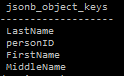
\includegraphics[scale=1]{sc/32}
\end{center}
\caption{Wynik zapytania z przykładu 2.}
\end{figure}%
Tu użyta funkcja jsonb\_object\_keys służy do wyekstrahowania kluczy z najbardziej zewnętrznego poziomu (zerowego poziomu zagnieżdżenia) dokumentu przekazanego.
\newpage
\subsubsection*{Przykład 3.}
\begin{lstlisting}[language=SQL,basicstyle=\footnotesize]
CREATE TYPE temp_person AS ("LastName" varchar(25), "personID" int, "FirstName" varchar(25), "MiddleName" varchar(25));
SELECT (jsonb_populate_record(null::temp_person,  data->'person')).* from public.personjsonb LIMIT 5;
\end{lstlisting}
\captionof{lstlisting}{Przykład 3.}\vspace{0.5cm}
\begin{figure}[h]
\begin{center}
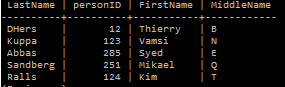
\includegraphics[scale=0.9]{sc/33}
\end{center}
\caption{Wynik zapytania z przykładu 3.}
\end{figure}%
Ten przykład pokazuje jak można przenieść dane z dokumentów do struktury tablicowej. W PostgreSQL możemy znaleźć kilka sposobów do takiego działania.
\subsubsection*{Przykład 4.}
\begin{lstlisting}[language=SQL,basicstyle=\footnotesize]
SELECT jsonb_array_elements(data->'email') from personjsonb;
\end{lstlisting}
\captionof{lstlisting}{Przykład 4.}\vspace{0.5cm}
\begin{figure}[h]
\begin{center}
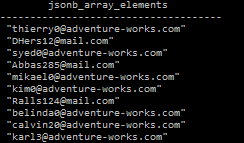
\includegraphics[scale=1]{sc/34}
\end{center}
\caption{Fragment wyniku zapytania z przykładu 4.}
\end{figure}%
Powyższy przykład pokazuje jak wyekstrahować wszystkie adresy e-mail ze wszystkich dokumentów. Warto zaznaczyć, że nie we wszystkich dokumentach znajduję się tablica "email", oraz długość tej tablicy w każdym dokumencie może wynieść 0, 1, 2. To oczywiście jest fragment wyników.
\subsubsection*{Przykład 5.}
\begin{lstlisting}[language=SQL,basicstyle=\footnotesize]
SELECT jsonb_typeof(data) AS Document, jsonb_typeof(data->'email') AS Email_Array, jsonb_typeof(data->'person'->'personID') AS PersonID, jsonb_typeof(data->'email'->0) AS Email, jsonb_typeof('true') AS Bool, jsonb_typeof('null') AS Null FROM personjsonb LIMIT 1;
\end{lstlisting}
\captionof{lstlisting}{Przykład 5.}\vspace{0.5cm}
\begin{figure}[h]
\begin{center}
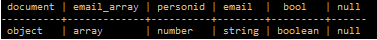
\includegraphics[scale=1]{sc/35}
\end{center}
\caption{Wynik zapytania z przykładu 5.}
\end{figure}%4

PostgreSQL daj nam możliwość sprawdzenia typów obiektów z dokumentu - jsonb\_typeof. Powyżej widzimy wszystkie możliwe typy danych w formacie JSON.
\newpage
\subsubsection*{Przykład 6.}
\begin{lstlisting}[language=SQL,basicstyle=\footnotesize]
BEGIN TRANSACTION;
SELECT jsonb_pretty(data) FROM public.personjsonb WHERE "ObjectID"=1922;
UPDATE public.personjsonb SET data = (SELECT jsonb_set(data,'{email,1}','"newmail@hotmail.com"',false) FROM public.personjsonb WHERE "ObjectID"=1922) WHERE "ObjectID"=1922;
SELECT jsonb_pretty(data) FROM public.personjsonb WHERE "ObjectID"=1922;
ROLLBACK;
\end{lstlisting}
\captionof{lstlisting}{Przykład 6.}\vspace{0.65cm}
\begin{minipage}{0.5\textwidth}
\makeatletter
\def\@captype{figure}
\makeatother
\begin{center}
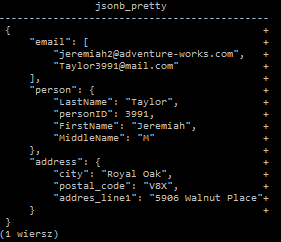
\includegraphics[scale=1]{sc/36}
\caption{Przed modyfikacją}
\end{center}

\end{minipage}
\begin{minipage}{0.5\textwidth}
\makeatletter
\def\@captype{figure}
\makeatother
\begin{center}
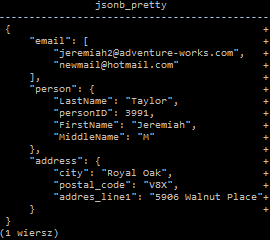
\includegraphics[scale=1]{sc/37}
\caption{Po modyfikacji}
\end{center}
\end{minipage}
\vspace{0.5cm}\newline
Powyżej widzimy chyba najważniejszą z funkcji przetwarzających - jsonb\_set. Równie ważna jest funkcja jsonb\_insert. Obie są dostępne tylko dla typu jsonb. Pierwsza z nich:
\begin{center}
jsonb\_set(dokument, '{scieżka}', 'nowy element', dodać\_nowy = true) 
\end{center}
Jej działanie polega na zmianie elementu znalezionego w przekazanej ścieżce na 'nowy element'. Jeśli dokument nie zawiera takiej ścieżki i dodać\_nowy jest true to dodana zostanie nowa para "klucz":"wartość".

\begin{center}
jsonb\_insert(dokument, '{scieżka}', 'nowy element', wstaw\_za = false) 
\end{center}
Ta metoda ma za zadanie dodawania wartości do tablicy.
W wypadku wcześniejszej funkcji istnieje możliwość jedynie dodania elementu na koniec tablicy, tu możemy wstawić go wszędzie w tablicy. O miejscu czy wstawiamy go przed, czy po wskazanej ścieżce decyduje parametr wstaw\_za.
\newpage
\subsection{Funkcje tworzące dokument JSON}
Oprócz funkcji przetwarzających PostgreSQL dysponuje drugą grupą funkcji służącą do konwersji różnego rodzaju danych do typów jsonb i json. Funkcjonalność ta jest przydatna wtedy, gdy posiadamy bazę relacyjną, a w aplikacji np. webowej wymieniamy dane przy pomocy technologii AJAX (AJAJ). Postgres daje nam do dyspozycji kilka różnych algorytmów przemiany danych w format dokumentu JSON. Oto kilka przykładów: 
\subsubsection*{Przykład 1.}
\begin{lstlisting}[language=SQL,basicstyle=\footnotesize]
SELECT to_jsonb(Name),Name FROM Users LIMIT 4;
SELECT to_jsonb(ARRAY(SELECT Name From Users LIMIT 4));
\end{lstlisting}
\captionof{lstlisting}{Przykład 1.}\vspace{0.65cm}

\begin{minipage}{0.5\textwidth}
\makeatletter
\def\@captype{figure}
\makeatother
\begin{center}
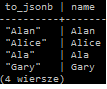
\includegraphics[scale=1]{sc/41}
\caption{Zapytanie nr. 1}
\end{center}

\end{minipage}
\begin{minipage}{0.5\textwidth}
\makeatletter
\def\@captype{figure}
\makeatother
\begin{center}
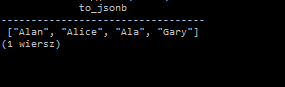
\includegraphics[scale=1]{sc/42}
\caption{Zapytanie nr. 2}
\end{center}
\end{minipage}
\vspace{0.5cm}\newline
Funkcje to\_jsonb() oraz odpowiadająca jej to\_json() konwertują przekazany parametr do odpowiadającego mu typu w formacie JSON. Powyżej widzimy konwersje stringu i tablicy.

\subsubsection*{Przykład 2.}
\begin{lstlisting}[language=SQL,basicstyle=\footnotesize]
SELECT array_to_json(ARRAY(SELECT idUsers From Users));
\end{lstlisting}
\captionof{lstlisting}{Przykład 2.}\vspace{0.5cm}

\begin{figure}[h]
\begin{center}
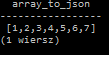
\includegraphics[scale=1]{sc/43}
\end{center}
\caption{Wynik zapytania z przykładu 2.}
\end{figure}%
Funkcja w tym przykładzie jest przeznaczona tylko dla tablic. Ten sam efekt można by otrzymać przy pomocy to\_json().

\subsubsection*{Przykład 3.}
\begin{lstlisting}[language=SQL,basicstyle=\footnotesize]
SELECT row_to_json(row,true) FROM (SELECT idUsers,username, Name, Surname, mail FROM Users WHERE idUsers=4) row;
\end{lstlisting}
\captionof{lstlisting}{Przykład 3.}\vspace{0.5cm}
\begin{figure}[h]
\begin{center}
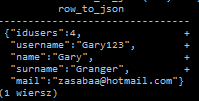
\includegraphics[scale=1]{sc/44}
\end{center}
\caption{Wynik zapytania z przykładu 3.}

\end{figure}%
Powyżej widzimy już trochę bardziej skomplikowane przekształcenie. Konwersja całej krotki do obiektu JSON może być całkiem użyteczna. Funkcja jako klucze do wartości z wiersza tablicy przypisuje nazwy atrybutów. Wartość logiczna przekazywana do funkcji row\_to\_json decyduje o sposobie formatowania, tzw. pretty\_bool.


\subsubsection*{Przykład 4.}
\begin{lstlisting}[language=SQL,basicstyle=\footnotesize]
SELECT json_build_array(ARRAY(SELECT Name From Users), ARRAY(SELECT idUsers From Users));
\end{lstlisting}
\captionof{lstlisting}{Przykład 4.}\vspace{0.5cm}
\begin{figure}[h]
\begin{center}
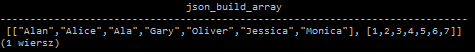
\includegraphics[scale=1]{sc/45}
\end{center}
\caption{Wynik zapytania z przykładu 4.}
\end{figure}%
Funkcja json\_build\_array służy do budowania trochę bardziej wyrafinowanych tablic.

\subsubsection*{Przykład 5.}
\begin{lstlisting}[language=SQL,basicstyle=\footnotesize]
SELECT jsonb_pretty(jsonb_build_object('FirstName',Name,'LastName',Surname,'City',Town,'ID', idUsers)) FROM Users WHERE idUsers=5;
\end{lstlisting}
\captionof{lstlisting}{Przykład 5.}\vspace{0.5cm}
\begin{figure}[h]
\begin{center}
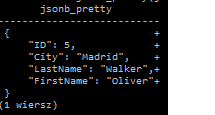
\includegraphics[scale=1]{sc/46}
\end{center}
\caption{Wynik zapytania z przykładu 5.}
\end{figure}%
Funkcja jsonb\_build\_object wydaje się najbardziej pożądana, służy do tworzenia obiektów typu jsonb (jest również jej odpowiednik dla typu json), w których sami możemy nadawać nazwy kluczy.


\newpage
\subsection{Tworzenie indeksów w dokumentach JSON}
Wspomnianym już wcześniej atutem typu jsonb jest możliwość utworzenia indeksów na kluczach dokumentu JSON. PostgreSQL daje nam do dyspozycji kilka metod indeksowania między innymi: B-tree, Hash, GIN. W przypadkach, gdy użytkownik nie podaje metody użyta zostaję B-tree (tak jak w poniższym przykładzie). Wszystkie metody działają na kluczach dokumentu JSON.
\subsubsection*{Przykład}
\begin{lstlisting}[language=SQL,basicstyle=\footnotesize]
SELECT "ObjectID", data->'person'->>'LastName'::text AS Surname FROM personjsonb WHERE data->'person'->>'LastName'::text LIKE 'T%';
CREATE INDEX surname on personjsonb (((data->'person'->>'LastName')::text));
SELECT "ObjectID", data->'person'->>'LastName'::text AS Surname FROM personjsonb WHERE data->'person'->>'LastName'::text LIKE 'T%';
\end{lstlisting}
\captionof{lstlisting}{Zapytanie testowe przed i po utworzeniu indeksu}\vspace{0.5cm}
W przykładzie sprawdzam czas wykonania zapytania przed i po utworzeniu indeksu. Zapytanie wykonuje dziesięciokrotnie i wyliczam średnią arytmetyczną. Realizuje to przy pomocy skryptu Python:
\begin{lstlisting}[language=Python,basicstyle=\footnotesize]
def test2():
	t = []
	query = "SELECT \"ObjectID\", data->'person'->>'LastName'::text AS Surname FROM personjsonb WHERE data->'person'->>'LastName'::text LIKE 'T%';"
	query_c = "CREATE INDEX surname on personjsonb (((data->'person'->>'LastName')::text));"
	query_d = "DROP INDEX surname"
	conn1 = psycopg2.connect(database="Inz", user="postgres", password="Password", host="127.0.0.1", port="5433")
	cur1 = conn1.cursor()
	t0 = time.time()
	for i in range(10):
		cur1.execute(query)
	t1 = time.time()
	t.append((t1-t0)/10)
	cur1.execute(query_c)
	conn1.commit()
	t0 = time.time()
	for i in range(10):
		cur1.execute(query)
	t1 = time.time()
	t.append((t1-t0)/10)
	f=open('test2.dat', "w")
	f.write(str(t)+"\n")
	f.close()
	cur1.execute(query_d)
	conn1.commit()
\end{lstlisting}
\captionof{lstlisting}{Funkcja testująca indeksy w Pythonie}\vspace{0.5cm} \newpage
Oto otrzymany wynik:
\begin{figure}[h]
\begin{center}
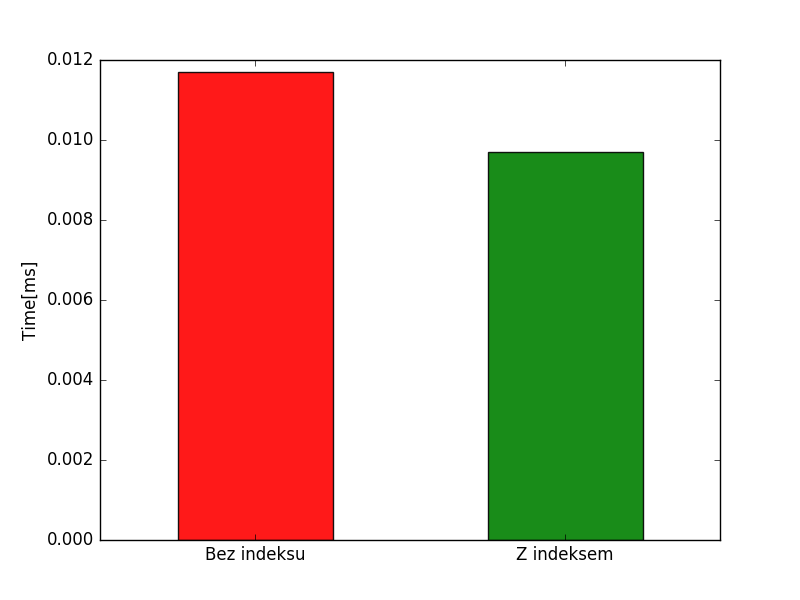
\includegraphics[scale=0.7]{ax/figindex}
\end{center}
\caption{Czas wykonania przykładowego zapytania z użyciem i bez użycia indeksu}
\end{figure}

Na podstawie wykresu widać minimalny wzrost wydajności w przypadku użycia indeksów.
\newpage
\section{Bazy dokumentowe}
\setlength{\parskip}{1\bigskipamount plus \smallskipamount minus \smallskipamount}
\subsection{Couchbase Server}
Couchbase Server jest wieloplatformowym narzędziem służącym do zarządzania nierelacyjną, dokumentową bazą danych. System pojawił się na rynku w 2010 roku. Wtedy był znany jako Membase Server.\cite{cdb} Wśród twórców tego oprogramowania znajdują się osoby współtworzące technologię memcached, której założeniem jest przechowywanie danych w pamięci RAM, co w znacznym stopniu zwiększa wydajność pracy. Takie rozwiązanie jest wspierane również przez omawiane narzędzie, chociaż Couchbase ma możliwość przechowywania danych na rzeczywistych dyskach.

Do zarządzania naszym serwerem mamy do dyspozycji przeglądarkowy interfejs, a także wersję konsolową cbq. W ramach serwera możemy tworzyć kilka węzłów, na których tworzy się pojemniki na dane (ang.\textit{ Data Buckets}), do których możemy przypisać pamięć RAM, która ma zarządzać pojemnikiem. Couchbase przechowuję dane w postaci dokumentów JSON.
\subsubsection{N1QL}
Bezapelacyjną zaletą Couchbase Server jest język N1QL, który służy do zarządzania dokumentami w bazie. Jego składnia jest bliźniacza do języka SQL. 
Utworzyłem pojemnik `Person\_Bucket` z dokumentami JSON (zestaw pierwszy przy prezentacji PostgreSQL). W Couchbase Server mamy możliwość wyboru dwóch rodzajów pojemników - Couchbase Bucket i Memcached Bucket. Pierwszy rodzaj zapisuję dane na dyskach, a drugi używa tylko pamięci RAM, jednak tylko ten pierwszy wspiera zapytania N1QL, dlatego go wybrałem. Oto przykładowe polecenia w N1QL:
\subsubsection*{Przykład 1.}
\begin{lstlisting}[language=SQL,basicstyle=\footnotesize]
CREATE PRIMARY INDEX `person_index` ON `Person_Bucket` USING VIEW;
\end{lstlisting}
\captionof{lstlisting}{Przykład 1.}\vspace{0.5cm}
W celu umożliwienia przeszukiwania pojemnika, należy utworzyć na nim indeks główny.
\subsubsection*{Przykład 2.}
\begin{lstlisting}[language=SQL,basicstyle=\footnotesize]
SELECT count(person) FROM `Person_Bucket`;
\end{lstlisting}
\captionof{lstlisting}{Przykład 2.}\vspace{0.5cm}
Proste zliczenie dokumentów w pojemniku.
\subsubsection*{Przykład 3.}
\begin{lstlisting}[language=SQL,basicstyle=\footnotesize]
SELECT person.LastName, count(person.LastName) FROM `Person_Bucket` GROUP BY person.LastName;
\end{lstlisting}
\captionof{lstlisting}{Przykład 3.}\vspace{0.5cm}
Zgrupowanie przy pomocy wartości klucza "LastName" znajdującego się w dokumencie zagnieżdżonym "person" i zliczenie liczby ich wystąpienia.
\subsubsection*{Przykład 4.}
\begin{lstlisting}[language=SQL,basicstyle=\footnotesize]
SELECT DISTINCT address.city AS City FROM `Person_Bucket` ORDER BY City ASC;
\end{lstlisting}
\captionof{lstlisting}{Przykład 4.}\vspace{0.5cm}
Wyselekcjonowanie unikalnych wartości klucza "city" i posortowanie ich.
\subsubsection*{Przykład 5.}
\begin{lstlisting}[language=SQL,basicstyle=\footnotesize]
SELECT person.LastName FROM `Person_Bucket` WHERE person.LastName LIKE 'T%' AND ARRAY_COUNT(email)=2;
\end{lstlisting}
\captionof{lstlisting}{Przykład 5.}\vspace{0.5cm}
\begin{figure}[h]
\begin{center}
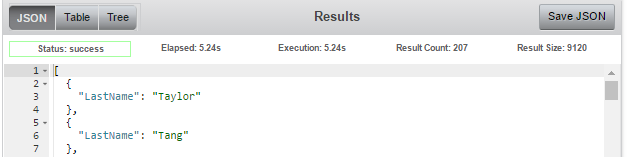
\includegraphics[scale=0.9]{sc/51}

\end{center}
\caption{Fragment wyniku zapytania z przykładu 5.}
\end{figure}\vspace{0.2cm}

Selekcja wartości klucza "LastName" w wypadku, gdy zaczyna się od 'T' i rozmiar tablicy "email" w danym dokumencie wynosi 2.
\subsubsection*{Przykład 6.}
\begin{lstlisting}[language=SQL,basicstyle=\footnotesize]
SELECT person, address FROM `Person_Bucket` WHERE email IS MISSING;
\end{lstlisting}
\captionof{lstlisting}{Przykład 6.}\vspace{0.5cm}
Selekcja dokumentów zagnieżdżonych "person" i "address" w wypadku, gdy w danym dokumencie nie istniej klucz "email".
\subsubsection*{Przykład 7.}
\begin{lstlisting}[language=SQL,basicstyle=\footnotesize]
UPDATE `Person_Bucket` i SET i.email = [i.person.LastName||'@new.pl'] WHERE email IS MISSING LIMIT 3 RETURNING i;
\end{lstlisting}
\captionof{lstlisting}{Przykład 7.}\vspace{0.5cm}
Dodanie tablicy o kluczu "email" do dokumentów, gdzie ten klucz nie występuje. W tablicy znajduje się adres e-mail wygenerowany na podstawie klucza "LastName". Dodatkowo występuje klauzula LIMIT 3 - aktualizacja w maksymalnie trzech dokumentach.
\subsubsection*{Przykład 8.}
\begin{lstlisting}[language=SQL,basicstyle=\footnotesize]
DELETE FROM `Person_Bucket` WHERE person.personID >= 18000;
\end{lstlisting}
\captionof{lstlisting}{Przykład 8.}\vspace{0.5cm}
Usuwanie dokumentów z pojemnika, których wartość klucza "personID" jest większa, bądź równa 18000.
\newpage
W powyższych zapytaniach widzimy, że do zagłębiania w głąb dokumentów JSON używa się kropki. Można tam dostrzec również przykładowe funkcje oraz operatory do przetwarzania tychże dokumentów (ARRAY\_COUNT(), IS MISSING). Istotną różnicą pomiędzy SQL, a N1QL jest format zwróconych danych. W przypadku SQL dane zwracane są jako tabela, a w drugim wypadku jako dokument, lub zbiór dokumentów JSON.




\subsection{MongoDB}
MongoDB to system zarządzania dokumentową bazą danych. Podobnie jak omawiany wcześniej Couchbase Server jest wieloplatformowym i darmowym rozwiązaniem No SQL-owym. Dane przechowywane są w kolekcjach, do których dodaje się dokumenty w formacie JSON. Te dokumenty przechowywane są w postaci BSON (ang. \textit{ Binary JSON}), czyli odpowiedniku jsonb z PostgreSQL. Pierwsza wersja oprogramowania została wydana w 2009 i od tego momentu deweloperzy poczynili duży postęp nad wydajnością i możliwościami systemu.\cite{mdb} Obecnie MongoDB jest jedną z popularniejszych baz dokumentowych na rynku. Tak samo jak omawiane wcześniej rozwiązanie MongoDB wspiera replikacje danych oraz pozwala na horyzontalne skalowanie.

Do obsługi serwera mamy do dyspozycji kilka możliwości, między innymi konsole mongo, a także graficzne interfejsy takie jak Robomongo, czy adminMongo.
\subsubsection{Przeszukiwanie kolekcji}
Do przeszukiwania i przetwarzania danych MongoDB dysponuje własnym podejściem, które jest odrębne od prezentowanego w przypadku PostgreSQL SQL-a. Po utworzeniu kolekcji i zaimportowaniu do niej dokumentów mamy w zanadrzu kilkanaście funkcji, które wykonujemy bezpośrednio na kolekcji. Oto kilka z nich: find(), group(), insert(), aggregate(), update(), remove(). Kolekcja person\_col zawiera te same dokumenty co Person\_Bucket z Couchbase Server. Poniżej znajdują się przykładowe zapytania, realizujące to co przykłady prezentowane dla CouchbaseServer:
\subsubsection*{Przykład 1.}
\begin{lstlisting}[language=SQL,basicstyle=\footnotesize]
db.person_col.find().count();
\end{lstlisting}
\captionof{lstlisting}{Przykład 1.}\vspace{0.5cm}
Zliczenie dokumentów w kolekcji.
\subsubsection*{Przykład 2.}
\begin{lstlisting}[language=SQL,basicstyle=\footnotesize]
db.person_col.aggregate([{"$group" : {_id:"$person.LastName", count:{$sum:1}}}])
\end{lstlisting}
\captionof{lstlisting}{Przykład 2.}\vspace{0.5cm}
Grupowanie po wartościach klucza "LastName" i zliczenie ich wystąpienia.
\newpage
\subsubsection*{Przykład 3.}
\begin{lstlisting}[language=SQL,basicstyle=\footnotesize]
db.person_col.distinct("addres.city").sort();
\end{lstlisting}
\captionof{lstlisting}{Przykład 3.}\vspace{0.5cm}
Wyekstrahowanie posortowanej listy unikalnych wartości klucza "city".

\subsubsection*{Przykład 4.}
\begin{lstlisting}[language=SQL,basicstyle=\footnotesize]
db.person_col.find({"person.LastName": /T.*/, "email": {$size: 2 }},{"person.LastName":1}).pretty();
\end{lstlisting}
\captionof{lstlisting}{Przykład 4.}\vspace{0.5cm}
Wyszukanie wartości klucza "LastName", gdy zaczynają się od "T" i liczba adresów e-mail przypisanych do danego dokumentu wynosi 2.

\begin{figure}[h]
\begin{center}
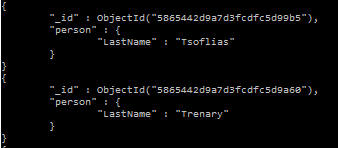
\includegraphics[scale=0.9]{sc/52}

\end{center}
\caption{Fragment wyniku zapytania z przykładu 4.}
\end{figure}
\subsubsection*{Przykład 5.}
\begin{lstlisting}[language=SQL,basicstyle=\footnotesize]
db.person_col.find({ "email": { $exists: null, $ne: true}},{person:1, address:1 });
\end{lstlisting}
\captionof{lstlisting}{Przykład 5.}\vspace{0.5cm}
Wyszukanie wartości dokumentów zagnieżdżonych "person" i "address", gdy w dokumencie głównym nie ma klucza "email".
\subsubsection*{Przykład 6.}
\begin{lstlisting}[language=SQL,basicstyle=\footnotesize]
db.person_col.find({"email": { $exists: null, $ne: true}}).limit(3).snapshot().forEach(
    function (elem) {
	db.person_col.update(
            { _id: elem._id },
            { $set: 
            	{  'email': [ elem.LastName +'@new.com']  }
});});
\end{lstlisting}
\captionof{lstlisting}{Przykład 6.}\vspace{0.5cm}
Dodanie do maksymalnie trzech dokumentów klucza "email" z przypisaną tablicą z adresem e-mail wygenerowanym na podstawie wartości klucza "LastName", gdy w danym dokumencie nie znajdował się wcześniej klucz "email".
\subsubsection*{Przykład 7.}
\begin{lstlisting}[language=SQL,basicstyle=\footnotesize]
db.person_col.remove({$where: "this.person.personID >= 18000"});
\end{lstlisting}
\captionof{lstlisting}{Przykład 7.}\vspace{0.5cm}
Usuwanie dokumentów z kolekcji, gdy wartość klucza "personID" jest większa, bądź równa 18000.

\noindent{Zapytania w MongoDB na samym początku mogą wydawać się bardzo skomplikowane, jednak w istocie często są łatwiejsze do napisania, niż te w SQL, czy N1QL. Na pewne w przypadku tego rozwiązania mamy w dyspozycji najwięcej różnego rodzaju operacji w stosunku do dokumentów JSON, niż w PostgreSQL i Couchbase. Ciekawą możliwością jest używanie kodu JavaScriptu wewnątrz zapytań (Przykład 6.).}

\setlength{\parskip}{0.5\bigskipamount plus \smallskipamount minus \smallskipamount}
\newpage
\subsection{Porównanie baz dokumentowych z PostgreSQL-em}
W pierwszej części tego zestawienia skupiłem na zestawieniu aspektów wydajnościowych. Jako zestaw testowy używam tego zbioru dokumentów JSON, który używałem przy prezentacji typów json i jsonb w  PostgreSQL-u - tabele personjson, personjsonb z Postgresa, pojemnik Person\_Bucket z Couchbase Server i kolekcja person\_col z MongoDB. Przygotowałem kilka przypadków testowych i zmierzyłem czas ich wykonywania w każdej z baz. Pierwszym przypadkiem jest wprowadzenie danych do każdej z baz. Kilka kolejnych to wydobycie danych oraz ich przetworzenia. Czasy wykonywania tych zapytań mierzyłem z poziomy skryptu napisanego w Pythonie z wyjątkiem zapytań w MongoDB, których wykonanie nadzorowałem z poziomu bazy. Ostatni przypadek testowy to sprawdzenie jak dużo miejsca na dysku zajmują przechowywane dane. Przy przypadkach testowych prezentuję zapytanie jakie jest testowane, krótki komentarz i wykres przedstawiający czas wykonanie lub rozmiar zajętego miejsca na dysku.
\subsubsection{Wprowadzenie danych}
\begin{lstlisting}[language=SQL,basicstyle=\footnotesize]
\i 'person_insert_jsonb.sql'
\i 'person_insert_json.sql'
mongoimport --db test --collection person_col --drop < person.json
cbdocloader -n localhost:8091 -u Administrator -p password -b Person_Bucket Person_Bucket.zip
\end{lstlisting}
\captionof{lstlisting}{Komendy wprowadzające dane}\vspace{0.5cm}
Długość wykonania dwóch pierwszych poleceń mierze bezpośrednio w bazie, natomiast dwa kolejne zwracają czas ich wykonania.
\begin{figure}[h]
\begin{center}
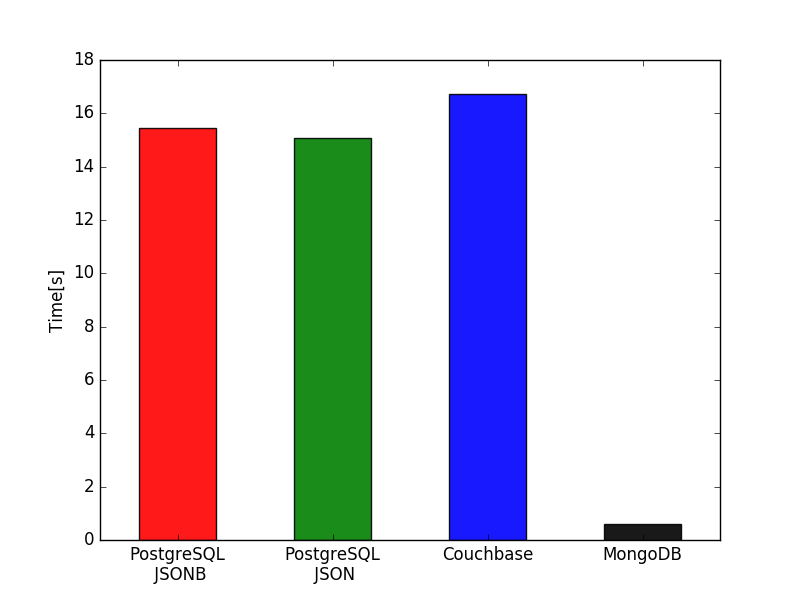
\includegraphics[scale=0.48]{ax/fig0}
\end{center}
\caption{Czas wprowadzania danych do poszczególnych baz}
\end{figure}
\subsubsection{Zapytania nr 1}
\begin{lstlisting}[language=SQL,basicstyle=\footnotesize]
SELECT max(cast(data->'person'->>'personID' AS int)) FROM personjsonb;
SELECT max(cast(data->'person'->>'personID' AS int)) FROM personjson;
SELECT max(person.personID) FROM `Person_Bucket`;
db.person_col.find({},{"person.personID":1}).sort({"person.personID": -1}).limit(1)
\end{lstlisting}
\captionof{lstlisting}{Pierwsza grupa zapytań}
\newpage
Cel zapytań: uzyskanie maksymalnej wartości klucza "personID" w dokumentach.
\begin{figure}[h]
\begin{center}
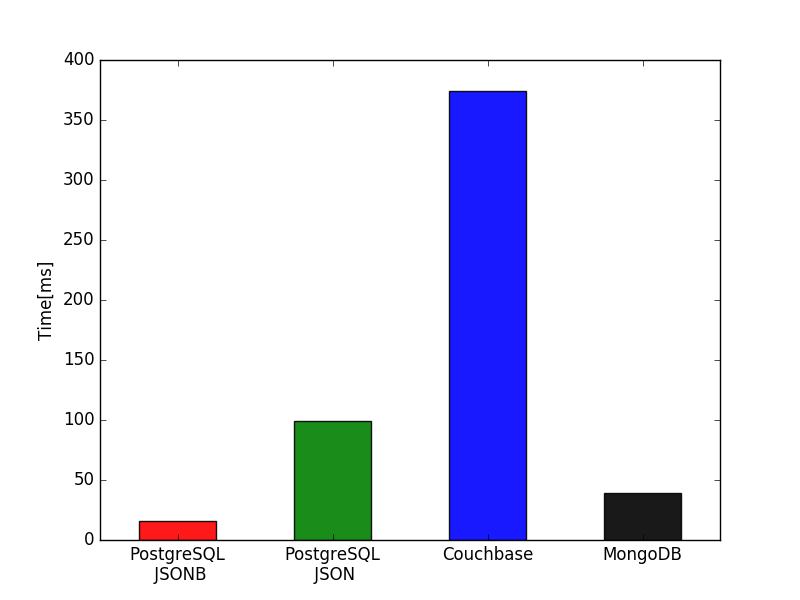
\includegraphics[scale=0.5]{ax/fig1}
\end{center}
\caption{Czas wykonania zapytań nr 1 w poszczególnych bazach}
\end{figure}

\subsubsection{Zapytania nr 2}
\begin{lstlisting}[language=SQL,basicstyle=\footnotesize]
SELECT data #> '{person,LastName}' AS NAME, COUNT(*) FROM public.personjsonb GROUP BY NAME;
SELECT data->'person'->>'LastName' AS NAME, COUNT(*) FROM public.personjson GROUP BY NAME;
SELECT person.LastName, count(person.LastName) FROM `Person_Bucket` GROUP BY person.LastName;
db.person_col.aggregate([{"$group" : {_id:"$person.LastName", count:{$sum:1}}}]);
\end{lstlisting}
\captionof{lstlisting}{Druga grupa zapytań}\vspace{0.5cm}
Cel zapytań: zgrupowanie przy użyciu wartości klucza "LastName" wraz z zliczeniem wystąpień wartości tego klucza.
\begin{figure}[h]
\begin{center}
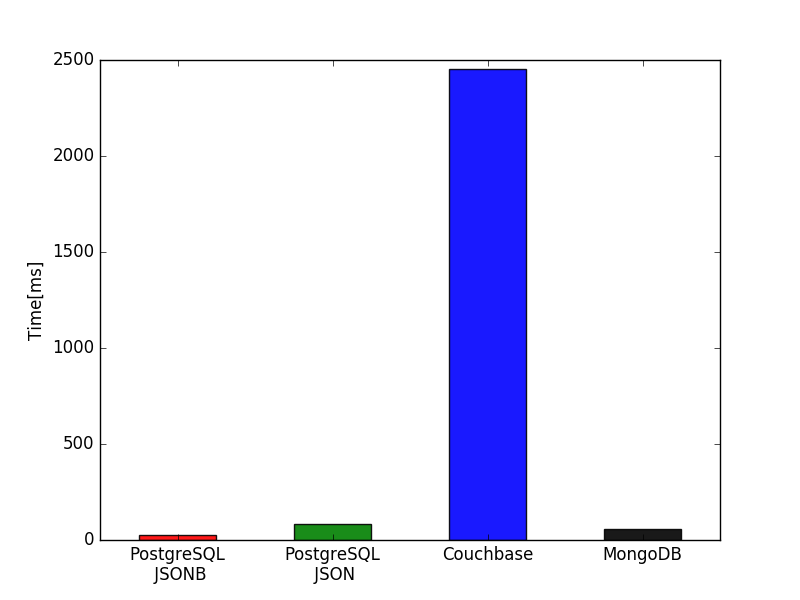
\includegraphics[scale=0.5]{ax/fig2}
\end{center}
\caption{Czas wykonania zapytań nr 2 w poszczególnych bazach}
\end{figure}
\newpage
\subsubsection{Zapytania nr 3}
\begin{lstlisting}[language=SQL,basicstyle=\footnotesize]
SELECT data FROM public.personjsonb WHERE data ? 'email';
SELECT data FROM public.personjson WHERE data::jsonb ? 'email';
SELECT data FROM `Person_Bucket` WHERE email IS NOT MISSING;
db.person_col.find({ "email": { $exists: true, $ne: null} });
\end{lstlisting}
\captionof{lstlisting}{Trzecia grupa zapytań}\vspace{0.5cm}
Cel zapytania: wyszukanie dokumentów, w których występuje klucz "email".
\begin{figure}[h]
\begin{center}
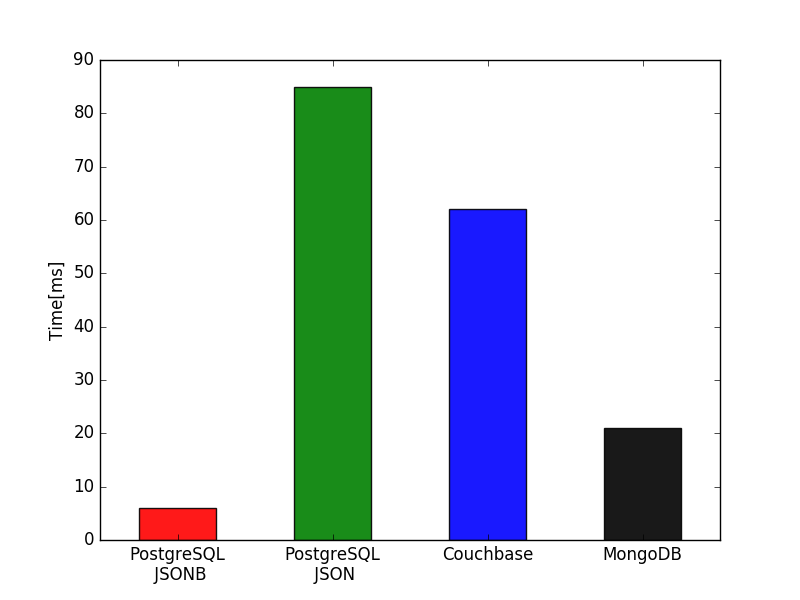
\includegraphics[scale=0.5]{ax/fig3}
\end{center}
\caption{Czas wykonania zapytań nr 3 w poszczególnych bazach}
\end{figure}

\subsubsection{Zapytania nr 4}
\begin{lstlisting}[language=SQL,basicstyle=\footnotesize]
SELECT "ObjectID", data->'person'->>'LastName' AS Surname FROM personjsonb WHERE data->'person'->>'LastName' LIKE 'T%' AND jsonb_array_length(data->'email')=2;
SELECT "ObjectID", data->'person'->>'LastName' AS Surname FROM personjson WHERE data->'person'->>'LastName' LIKE 'T%' AND json_array_length(data->'email')=2;
SELECT person.LastName FROM `Person_Bucket` WHERE person.LastName LIKE 'T%' AND ARRAY_COUNT(email)=2;
db.person_col.find({"person.LastName": /T.*/, "email": {$size: 2 }},{"person.LastName":1}).pretty();
\end{lstlisting}
\captionof{lstlisting}{Czwarta grupa zapytań}\vspace{0.5cm}
Cel zapytań: wyszukanie danych z dokumentów, gdzie wartość klucza "LastName" zaczyna się od "T" i długość tablicy "email" wynosi 2.
\begin{figure}[h]
\begin{center}
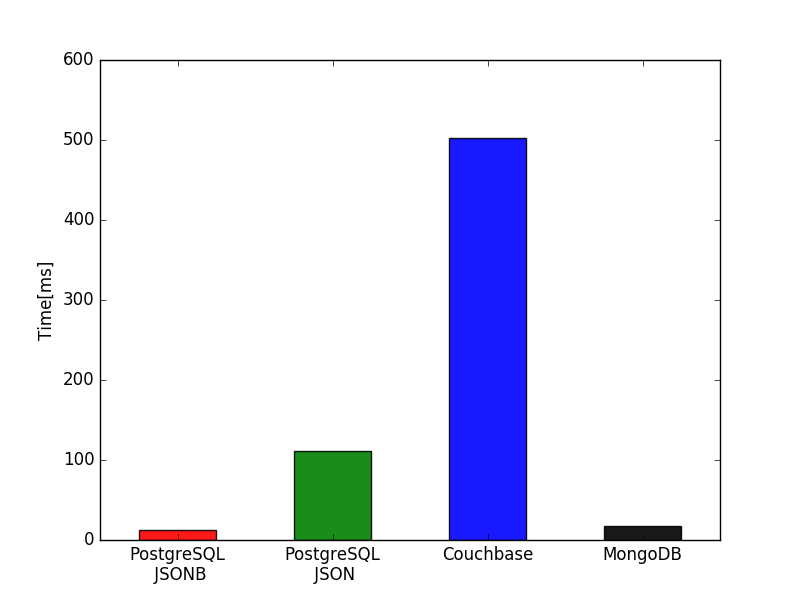
\includegraphics[scale=0.5]{ax/fig4}
\end{center}
\caption{Czas wykonania zapytań nr 4 w poszczególnych bazach}
\end{figure}
\newpage
\subsubsection{Zapytania nr 5}
\begin{lstlisting}[language=SQL,basicstyle=\footnotesize]
UPDATE public.personjsonb d SET data = (SELECT data || ('{"email":[' || quote_ident(dd.data->'person'->>'LastName'||'@hotmail.com')||']}')::jsonb  FROM public.personjsonb dd  WHERE d."ObjectID"=dd."ObjectID") WHERE not d.data ? 'email';
UPDATE public.personjson d SET data = (SELECT data::jsonb || ('{"email":[' || quote_ident(dd.data->'person'->>'LastName'||'@hotmail.com')||']}')::jsonb  FROM public.personjson dd  WHERE d."ObjectID"=dd."ObjectID")::json WHERE not d.data::jsonb ? 'email';
UPDATE `Person_Bucket` i SET i.email = [i.person.LastName||'@new.pl'] WHERE email IS MISSING;
db.person_col.find({"email": { $exists: null, $ne: true}}).snapshot().forEach( function (elem) {db.person_col.update({_id: elem._id },{ $set:{'email': [ elem.LastName +'@new.com']}});});
\end{lstlisting}
\captionof{lstlisting}{Piąta grupa zapytań}\vspace{0.5cm}
Cel zapytań: aktualizacja dokumentów, w których nie występuje klucz "email".

\begin{figure}[h]
\begin{center}
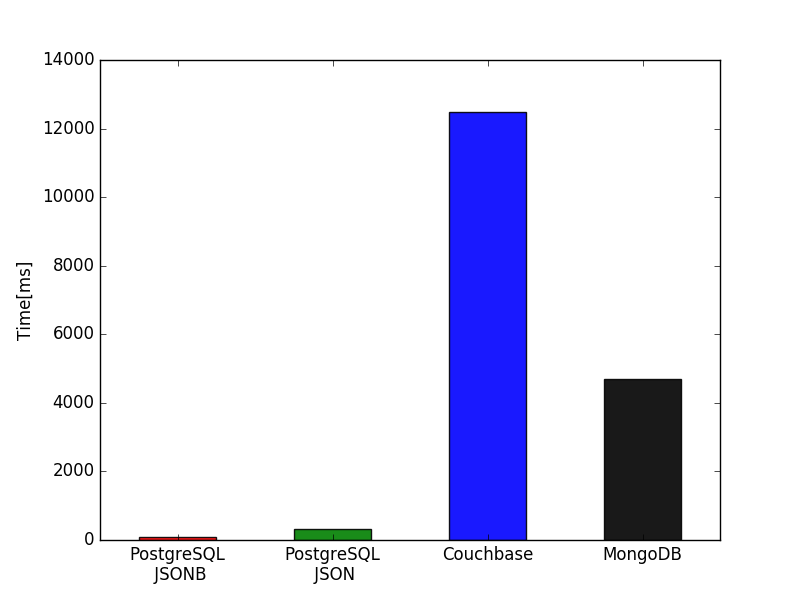
\includegraphics[scale=0.5]{ax/fig5}
\end{center}
\caption{Czas wykonania zapytań nr 5 w poszczególnych bazach}
\end{figure}

\subsubsection{Zapytanie nr 6}

\begin{lstlisting}[language=SQL,basicstyle=\footnotesize]
DELETE FROM personjsonb WHERE (cast(data->'person'->>'personID' AS int))>=18000;
DELETE FROM personjson WHERE (cast(data->'person'->>'personID' AS int))>=18000;
DELETE FROM `Person_Bucket` WHERE person.personID >= 18000;
db.person_col.remove({$where: "this.person.personID >= 18000"});
\end{lstlisting}
\captionof{lstlisting}{Szósta grupa zapytań}\vspace{0.5cm}
Cel zapytań: skasowanie dokumentów z bazy.
\begin{figure}[h]
\begin{center}
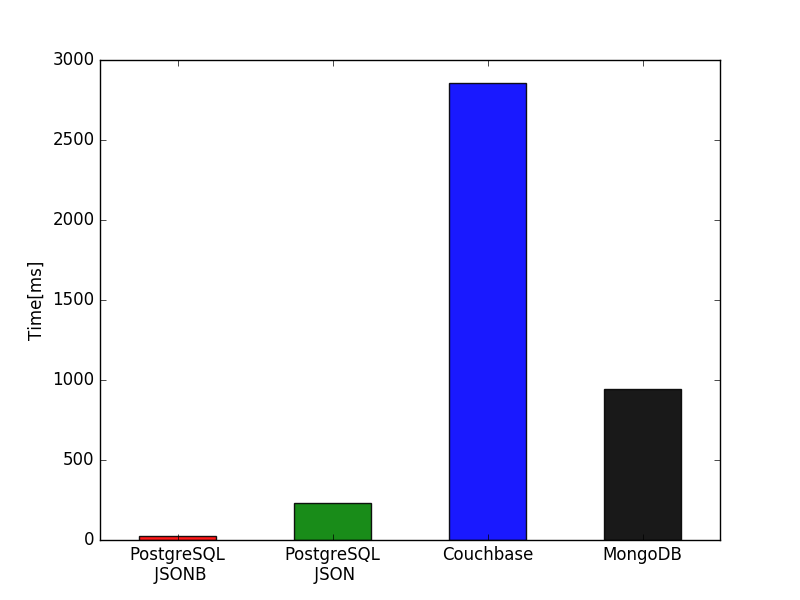
\includegraphics[scale=0.5]{ax/fig6}
\end{center}
\caption{Czas wykonania zapytań nr 6 w poszczególnych bazach}
\end{figure}

\subsubsection{Rozmiar na dysku}
\begin{figure}[h]
\begin{center}
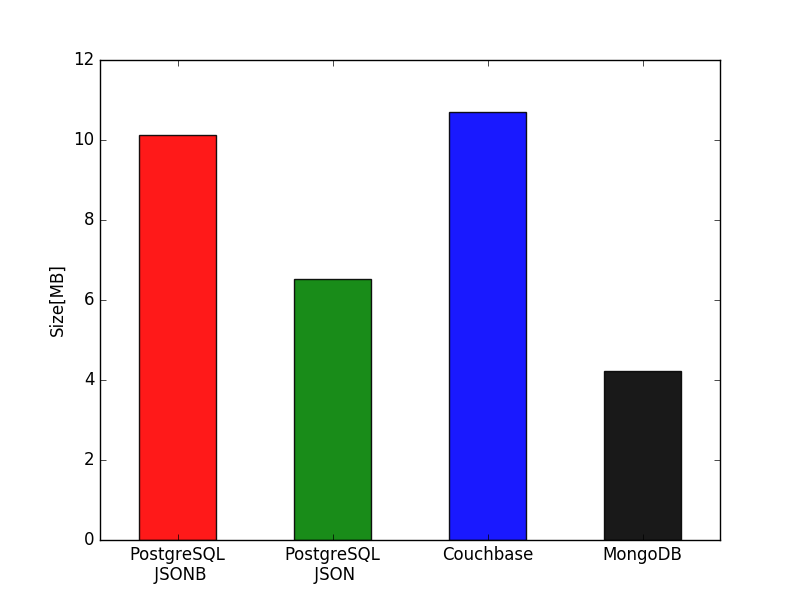
\includegraphics[scale=0.6]{ax/fig7}
\end{center}
\caption{Zajęty rozmiar na dysku w poszczególnych rozwiązaniach}
\end{figure}

\setlength{\parskip}{1.5\bigskipamount plus \smallskipamount minus \smallskipamount}
\newpage
\subsubsection{Podsumowanie wydajności}
Przedstawione wykresy dają nam dobry obraz działania przedstawionych baz. W przypadku wprowadzania danych zdecydowanym liderem okazała się baza MongoDB, która wyprzedza pozostałe rozwiązania. Potwierdziła się również przedstawiona wcześniej teza zgodnie, z którą json (PostgreSQL) jest szybszy we wprowadzaniu danych od jsonb (minimalnie), a wolniejszy w ich przetwarzaniu. Prawie we wszystkich testach najwolniej działał Couchbase, nawet pomimo stworzenia dodatkowych indeksów, jednak prawie wszystkie testy zakładały użycie N1QL, a więc zmuszony byłem do korzystania z Couchbase Bucket (alternatywą jest Memcached Bucket, który nie wspiera N1QL). Typ jsonb z PostgreSQL i baza MongoDB działają ze zbliżoną prędkością jeśli chodzi o przeszukiwanie danych i ich grupowanie, a json jest trochę wolniejszy. W aspekcie aktualizacji i kasowania danych najwydajniej pracuje Postgres. Ostatnim przypadkiem testowym był pomiar rozmiaru zajętego na dysku. Najkorzystniej wypadła baza MongoDB.

\noindent{
Podsumowując, MongoDB oraz jsonb z PostgreSQL działają porównywalnie. W niektórych przypadkach korzyść widać po jednej ze stron, a w innych po drugiej. Typ json z Postgresa jest wyraźniej wolniejszy od jsonb, więc w praktyce jest nieopłacalny. }

\subsubsection{Spojrzenie z innej strony}
Patrząc z punktu widzenia możliwości przetwarzania dokumentów JSON w przedstawionych bazach to tu widzę przewagę baz dokumentowych. Z pośród prezentowanych systemów największą gamą rozwiązań w tej kwestii dysponuje MongoDB. Inną pozytywną cechą wszystkich porównywanych wyżej baz jest możliwość tworzenia dodatkowych indeksów nawet na polach dokumentów, co zwiększałoby szybkość przeszukiwań.


\noindent{Pomijając aspekty wydajnościowe, przy decyzji o postawieniu na konkretny rodzaj bazy, mając w zanadrzu czysto dokumentową i relacyjną z typem obsługującym dokumenty należy rozważyć konsekwencje takiego wyboru. Z jednej strony obsługa transakcji może być niezbędna, albo pomysł, aby wkomponować dokumenty w model relacyjny może być kuszący, jednak należy pamiętać, że funkcjonalność odnosząca się do tychże dokumentów, którą oferują bazy czysto dokumentowe jest znacznie większa, niż w modelu relacyjnym. Dodatkowo nie można zapominać o głównym atucie podejścia nierelacyjnego - skalowalności horyzontalnej.}
\newgeometry{
 a4paper,
 total={170mm,257mm},
 left=20mm,
 top=20mm,
 right=10mm,
 bottom=2cm,
 nohead
 }
\newpage

\section{Bibliografia}

\begingroup
\renewcommand{\section}[2]{}%
\begin{thebibliography}{}
\bibitem{p} PostgreSQL Documentaion: https://www.postgresql.org/docs/ 
\bibitem{mdb} MongoDB Documentation: https://docs.mongodb.com/ 
\bibitem{cdb} Couchbase Server Documentation: https://developer.couchbase.com/
\bibitem{nosql} NoSQL: http://nosql-database.org/
\bibitem{ll1} Piotr Zieliński: \emph{Wprowadzenie do NoSQL}, https://msdn.microsoft.com/pl-pl/dn912483.aspx (22.12.2016)

\bibitem{l3} A Timeline of Database History : http://www.quickbase.com/articles/timeline-of-database-history (28.12.2016)
\bibitem{b1} Dan Sullivan:
\emph{NoSQL For Mere Mortals}, Helion 2015, ISBN: 978-83-283-2488-6

\bibitem{l1} https://www.quora.com/What-is-the-relation-between-SQL-NoSQL-the-CAP-theorem-and-ACID (22.12.2016)
\bibitem{js} http://www.json.org/json-pl.html (18.12.2016)

\end{thebibliography}


\end{document}

